\documentclass[pdftex,10pt,a4paper,oneside]{report}

\usepackage{amsmath}
\usepackage{algorithm}
\usepackage{algorithmic}
\usepackage{fancyhdr}
\usepackage{graphicx}
\usepackage{lipsum}
\usepackage{multirow}
\usepackage{setspace}
\usepackage{verbatim}
\usepackage{tabularx}
\usepackage{ltablex}
\usepackage{graphicx}
\usepackage{listings}
\usepackage{xcolor}
\usepackage{hyperref}
\fancyhf{}
\pagestyle{fancy}
\renewcommand{\headrulewidth}{0.2pt}
\lstdefinestyle{mystyle}{
    backgroundcolor=\color{lightgray!20}, % Background color
    commentstyle=\color{green},           % Comment style
    keywordstyle=\color{blue},            % Keyword style
    numberstyle=\tiny\color{gray},        % Line number style
    stringstyle=\color{red},              % String style
    basicstyle=\ttfamily\footnotesize,    % Basic font style
    breaklines=true,                      % Automatic line breaking
    numbers=left,                         % Line numbers on the left
    numbersep=5pt,                        % Distance of line numbers from the code
    frame=single,                         % Adds a frame around the code
    captionpos=b,                         % Position of the caption (bottom)
    showspaces=false,                     % Don't show spaces
    showstringspaces=false,               % Don't show spaces in strings
    showtabs=false,                       % Don't show tabs
    tabsize=2                             % Tab size
}
\lstset{
    style=mystyle,
    morekeywords={function, var, let, const, def}, % Add more keywords if needed
}
\lstdefinestyle{python}{
    language=Python,
    style=mystyle
}

\lstdefinestyle{javascript}{
    language=JavaScript,
    style=mystyle
}

% Styles can be Sonny, Lenny, Glenn, Conny, Rejne, Bjarne and Bjornstrup
\usepackage[Glenn]{fncychap} 

\begin{document}

% !TEX root =  ../Dissertation.tex

\thispagestyle{empty}

\begin{spacing}{2}
	\begin{center}
		
\includegraphics[scale = 1.5]{Preamble/BirmCrest.png}
	\end{center}
	\vspace{10mm}
	\begin{center}
		\textbf{\Large Adding retention techniques to daily games.}
		\vspace{20mm}
		\\\textbf{\Large Patrick Tierney-Lever}
		\vspace{30mm}
	\end{center}
	\begin{center}
		{\large School of Computer Science}
		\\ {\large College of Engineering and Physical Sciences}
		\\ {\large University of Birmingham}
		\\ {\large 2023-24}
	\end{center}
\end{spacing}

\pagenumbering{roman}



\chapter*{Abstract}
\addcontentsline{toc}{chapter}{Abstract}
This project explores the impact of retention techniques on user satisfaction and engagement within web applications, specifically targeting the daily game genre. The study involved developing two versions of a Wordle-like game: a basic version without retention features and an enhanced version, named The Gauntlet, which includes features like leaderboards, achievements, and extended functionality. Through comprehensive user surveys and detailed data analytics, it was demonstrated that The Gauntlet significantly outperformed the basic Wordle in terms of user satisfaction, engagement time, and retention rates. The findings suggest that integrating strategic retention techniques can greatly enhance user engagement. Future work could explore adaptive, personalized retention strategies to further optimize user satisfaction and long-term retention in web applications.
\clearpage
\begin{center}
    \Huge % Adjust the size as needed
    \textbf{Try it yourself:} \\
    \begin{figure}[h] % 'h' means 'here' - places the figure where it's defined
    \centering
    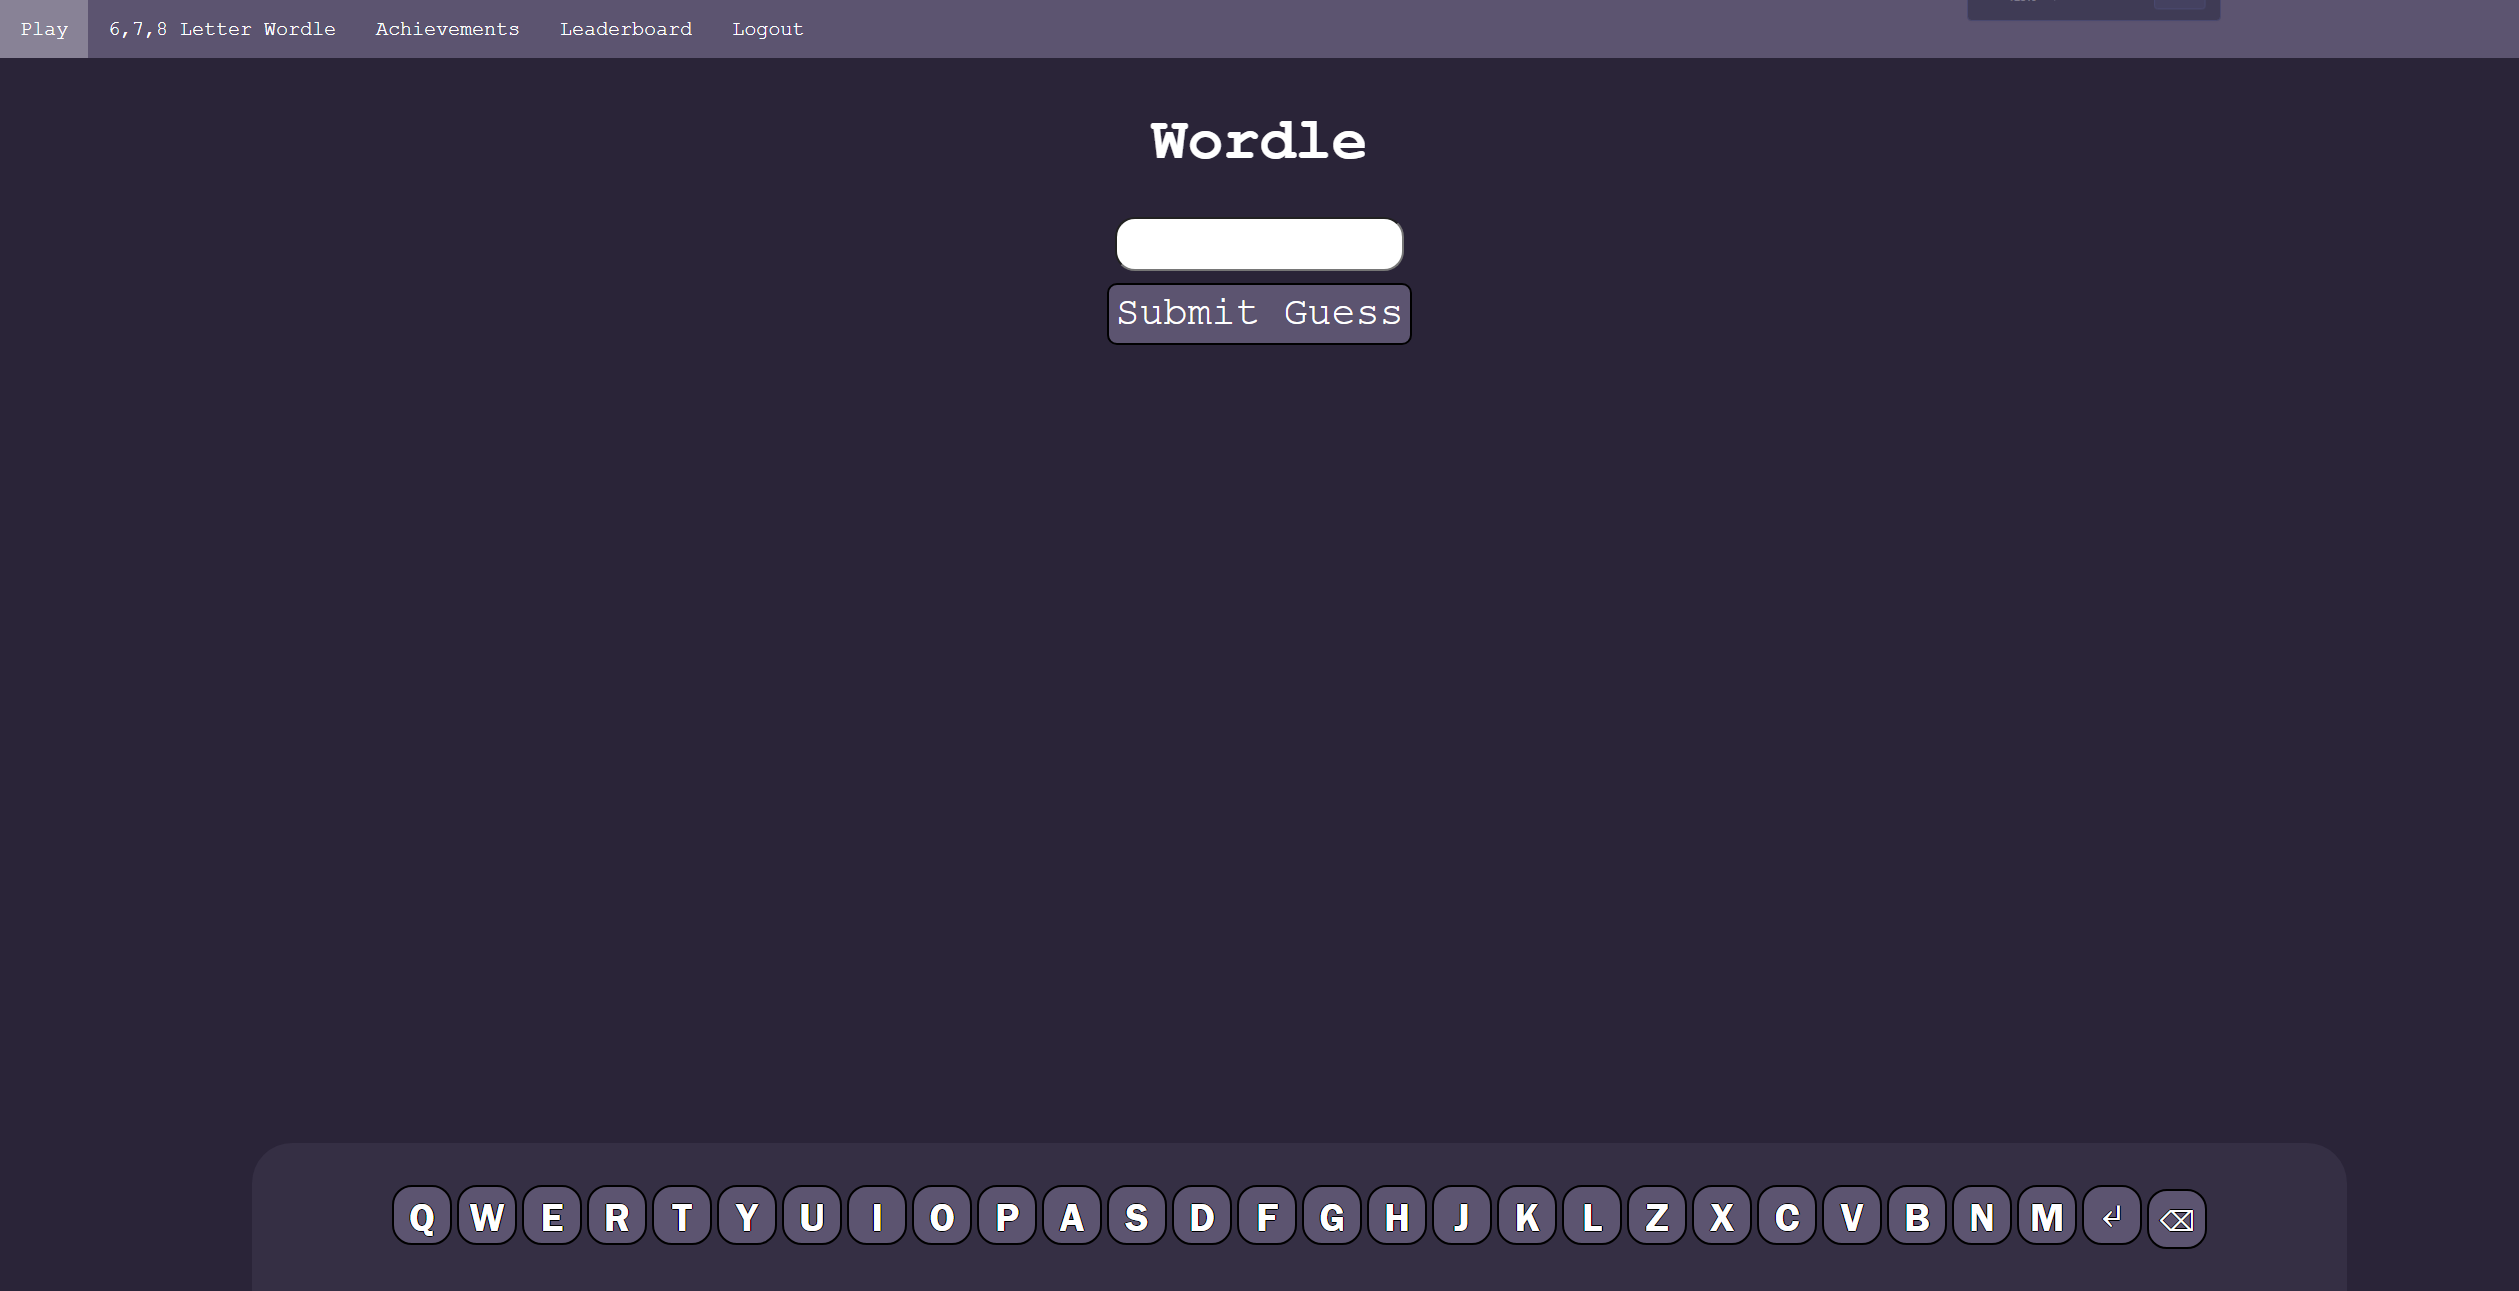
\includegraphics[width=\textwidth]{Picture_of_website.png} % Replace with your image file
    \label{fig:example}
    \end{figure}
    \vspace{1cm} % Adds some space between the text and the URLs

    \Large % Adjust the size as needed
    \texttt{\href{https://the-gauntlet-5a20b0d87ed3.herokuapp.com/wordle}{https://the-gauntlet-5a20b0d87ed3.herokuapp.com/wordle}} \\
    \vspace{0.5cm} % Adds some space between the two URLs
    \texttt{\href{https://wordle-no-login-c983e50c89bf.herokuapp.com}{https://wordle-no-login-c983e50c89bf.herokuapp.com}}
\end{center}
%\include{Preamble/Dedication} % Comment out for UG dissertations
%\include{Preamble/Declarations} % Comment out for UG dissertations
\include{Preamble/Contents}
\include{Preamble/ChapterMods}

% !TEX root =  ../Dissertation.tex

\chapter{Introduction}
In October 2021, Wordle was released and was a resounding success almost immediately after launch. The website grew traction quickly, going from only 90 players on November 1st to 300,000 on January 2nd 2022.\cite{Daniel2022} This success led to other developers working on games inspired by Wordle and has created a thriving community of smaller websites \cite{Adory2023} that follow in what will be referred to as the daily game genre of web application. The daily game genre has had continued success, but only a fraction of what Wordle has received.\cite{Google2024} Josh Wardle, the creator of Wordle, attributes much of the success of Wordle to the outreach of its shareable ‘emoji grid’  that was popular on Twitter early on in Wordle's conception.\cite{Slate2022} This was pivotal to bringing users to the website (which has since been acquired by NYT Games and added to their selection).\cite{nyt2022} However, once they gained this considerable player base, there was a lack of functionality that made players want to continue; the only thing that drew them back to the web application was the game itself. 

This project hypothesises that if retention techniques found in other multiplayer online games are added to the daily game genre of web applications \cite{Katkoff2016}, users will be more satisfied and retention will be increased. If the hypothesis is valid, developers in the daily game genre could augment their offerings to deliver a more engaging and exciting experience whilst increasing user retention.

To test this paper's hypothesis, there will be a self-conducted study of the effectiveness of these retention techniques by creating a simple Wordle clone, which will be referred to as Wordle no-login and a version of Wordle that has the retention techniques of more features, a leaderboard, and a set of achievements for participants to play, that will be named The Gauntlet. Users will be asked to complete two surveys, and with their permission, the web application will track the activity on their web browser to see if there is any increase in time spent and thus, engagement. The users will be asked to complete a survey when the testing is over to determine if they felt more satisfied using the website with increased functionality.
% !TEX root =  ../Dissertation.tex

\chapter{Literature Review}
User retention in gaming is a new topic of conversation in scholarship,\cite{Tseng2015} as retention was previously less critical to the gaming space.\cite{Petrovskaya2022} Now that the Free-to-Play (F2P) model is more prevalent \cite{Koskenvoima2015}, particularly in mobile gaming,\cite{Skorin-Kapov2022} having a user stay on longer increases their chances of making in-app purchases.\cite{Jang2021} However, these same concepts can be used to retain users and monetise them differently.\cite{Jung2022} The daily game genre of web applications tends to use advertisements to monetise their websites.\cite{Framed} Another way is through memberships to the website that can include benefits such as exclusive content, the ability to export and import your stats, and the ability to sync your stats for all of their other sites.\cite{Ko-fi}

Even with these monetisation approaches, user retention can still benefit this genre of web application.\cite{Ross2018} It is shown that a wider breadth of engagement with any content increases the chance of a user becoming a member.\cite{Yang2022} While the quality and trust of a website are not indicative of how many advertisements someone will click, as it is more based on the quality of the advert, the chance of a user clicking on an advert will naturally be linked with how much time a user spends on a website.\cite{Werner2022}

While it has been established that user retention is still important for web applications without micro-transactions, it is also necessary to decide what sort of user retention techniques are the strongest without adding unnecessary monetisation and keeping users satisfied.\cite{Ross2018} To find these techniques, World of Warcraft is a fitting start as they have been using a Games as a Service model (GaaS) for many years before the popularisation of F2P and mobile gaming. Thomas Debeauvais et al. have researched the retention mechanisms in World of Warcraft, and their research indicated two main techniques that are driving factors that retain players: achievement and social play.\cite{Debeauvais2010} The ‘hardcore’ players in World of Warcraft have higher playtime and, in surveys, were more interested in their gaming experience, having a challenge and a reward for their achievements. Casual players are more interested in the game's social aspect, which involves players grouping with their friends to take on challenges together.\cite{Debeauvais2010}

When researchers explore mobile play, these two retention techniques of ‘social’ and ‘achievement’ are consistent. Research has been done into the MMO World of Tanks players, which are also available as an app on mobile phones. The game is centred around armoured warfare, where players control a variety of tanks and engage in team-based battles. The game emphasises strategy, teamwork, and tactical combat rather than fast-paced action. When Liyang Gu et al. researched the World of Tanks replay system,\cite{Gu2021}, they found that while only a small number of users used this system, they tended to be more ‘hardcore’ players. This is because the replay communities surrounding this system mean that users felt a social aspect of the game and were more dedicated to playing. Immersion is something else in World of Tanks that affects user retention. A different paper by Liyang Gu et al. shows that users with a stronger sense of immersion in World of Tanks are also more likely to be retained.\cite{Gu2018} 

Paul Bertens et al. have made a scalable multidimensional churn prediction model that has been very accurate at predicting player churn.\cite{Bertens2017} One of the main input predictors for player churn is that the higher the level of the player, the less likely they are to churn. This indicates that the more a user feels they have achieved in a game, the more likely they will be retained for extended periods.\cite{Bertens2017}

Another retention technique is adding features, which can improve the number of users. However, it is essential to note that adding too many features can affect user acquisition, as a user may try to access your product and find it ‘overwhelming’ or ‘confusing,’ which may lead them to use another product.\cite{Hamilton2017}


\section{Ethics of Retention Techniques}
Various retention techniques have been studied and applied to online games. Some games have used these techniques, especially the more ethically dubious ones, to push their game to levels of addiction where players will find themselves spending an excessive amount of time on a game and often spending an excessive amount of money. A leading force behind this addiction that players can find themselves in is the retention techniques that have been applied to these games.\cite{Bernik2023}

A genre of game that has mastered retention techniques is ‘gacha games’. Gacha games are a genre primarily founded in Japan in the early 2010s. The etymology of the word ‘Gacha’ comes from the word ‘Gachapon’; these vending machines originated in Japan in the 1960s and dispensed different toys each time you paid.\cite{Bernik2023} Gacha games have continued that legacy by having in-game rewards that depend on random chance, which can be increased with in-app purchases of ‘tickets’ that will let you roll multiple times for a reward.\cite{Bernik2023}

Many have criticised Gacha games for their use of retention techniques as they bring gambling into the hands of younger players. While the ethics of this gameplay loop are questionable, its efficacy cannot be denied. miHoyo, one of the largest gacha game studios, has gone from a company with 15 million dollars of revenue in 2015 to 1.7 billion dollars in 2023.\cite{Pingwest2023} A large part of this is their use of the ‘free to play (F2P)’ and ‘games as a service (GaaS)’ models that heavily rely on retention techniques to keep their player base consistently returning to their game.\cite{Bernik2023}

Genshin Impact was one of MiHoyo's biggest games, recently overtaken by more recent titles but still making 60,500,000 USD in revenue in June 2024 and the game that introduced them to Western audiences.\cite{Gacha2024} It applies all the previously mentioned techniques: regular content updates, a gacha system, daily and weekly activities, wait-to-play, social features, progression, and reward systems. This led to massive success with both Asian and Western audiences.\cite{Greting2022}

Recent scholarship has pushed back against the use of these techniques. One of whom is Harry Brignull, a doctor in Cognitive Science who coined the phrase ‘dark patterns’ in his book "Deceptive Patterns: Exposing the Tricks Tech Companies Use to Control You" \cite{Brignull2023}. This phrase is often used in online discourse in video games like Genshin Impact. Harry Brignull argues that retention techniques like waiting to play, daily activities, and invested value intentionally manipulate cognitive biases to create an addiction and exploit the user for monetary gain.\cite{Brignull2023}

While this paper intends to advocate for the use of some retention techniques, it is essential to point out that the intention is not to create a version of Wordle that uses these ‘dark pattern’ retention techniques to the end of exploiting the user by intentionally making it too addictive nor should this be construed as an advocacy of the inclusion of microtransactions in the daily game genre of web applications. This paper advocates for a middle ground of adding proven retention techniques that increase user satisfaction and retention without adding these dark pattern techniques used in the gacha game genre to exploit the user for monetary gain. 

% !TEX root =  ../Dissertation.tex

\chapter{Design}

\section{Methodology}
\begin{figure}[h] % 'h' means 'here' - places the figure where it's defined
    \centering
    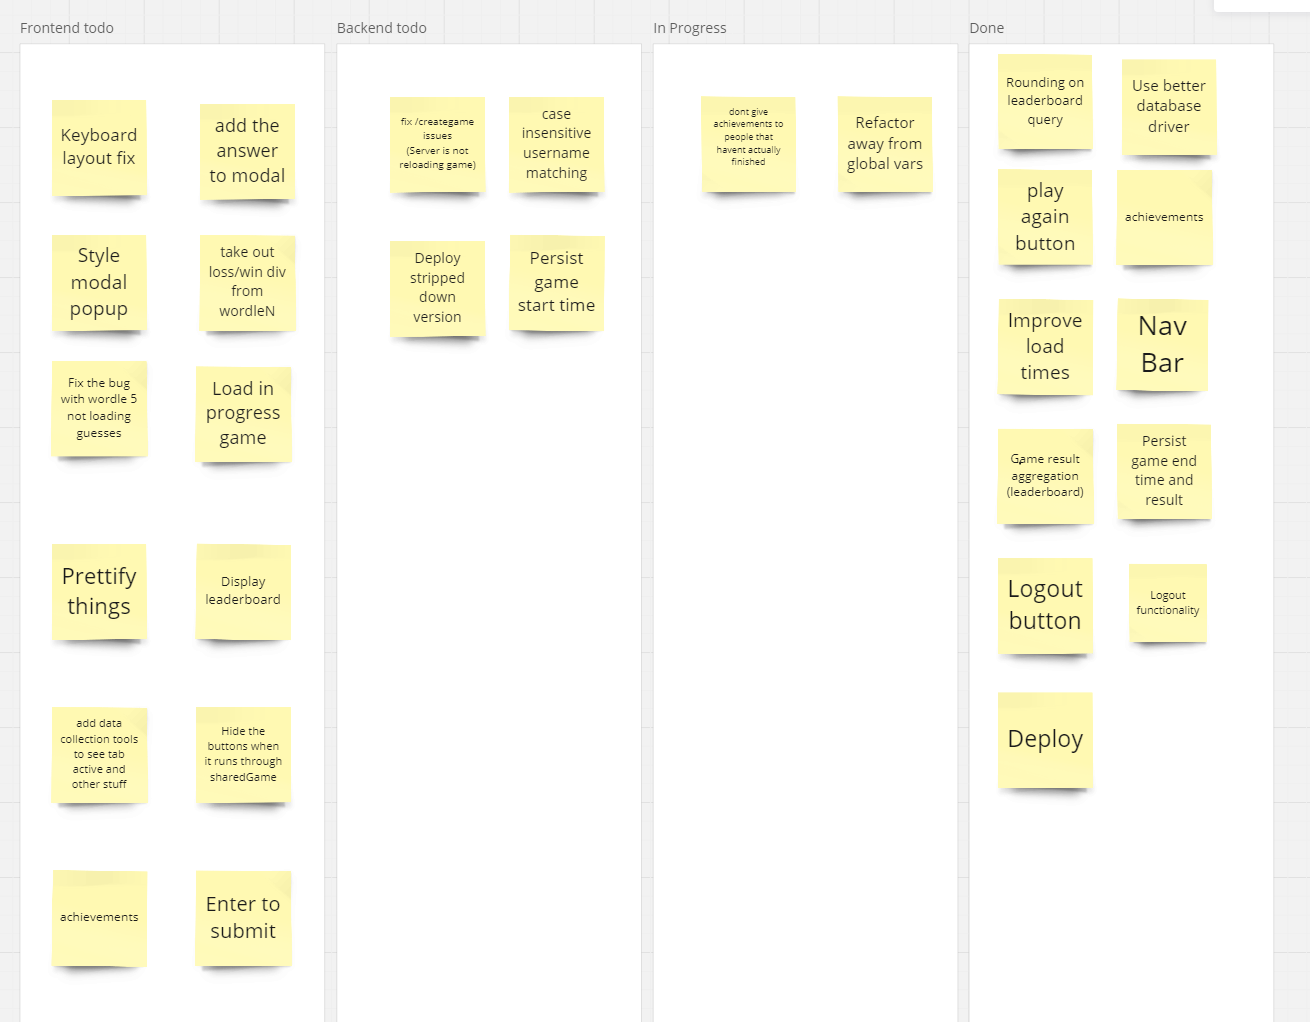
\includegraphics[width=\textwidth]{Kanban_Board.png} % Replace with your image file
    \caption{Kanban Board partway through production}
    \label{fig:example}
\end{figure}
While development was only finished by one person, it was pertinent to have a methodology to use while components were in development. For this, a Kanban approach was used,\cite{Toyota2021} using a web application called Miro. A project board with an essential to-do, in-progress, and finished workflow was created.\cite{Miro2024} The workflow limit was two, so there would only be that many in the in-progress swim lane simultaneously. 

This approach allowed the ability to focus on vertical slices of the product each time, which works in tandem with React's component approach to building functioning web applications and creating vertical slices of incremental value.\cite{Sarrion2023}

\section{Goals and Approach}
A participant in the later experiment was interviewed before development was started, particularly on the web application's retention techniques. The main goal of the interview was to understand what would make players want to return to a Wordle application and what made them leave in the first place. It was also important to identify which user retention techniques would feel most natural to the user to be incorporated into a daily game web application.

The interviewee was previously an avid player of Wordle when it was first released but had slowly stopped playing. They reasoned that they had gotten ‘tired’ of playing the same thing daily, especially when they found that they would always find the answer. They also found that after a certain amount of time, people stopped sending the emoji grid, showing users their daily score. 

While it is helpful to get ideas from users, sometimes a web application implements a feature that a user was unaware they would want until it was implemented. The user was presented with a list of retention techniques and asked to select their preferred option.

Different retention techniques, such as a daily reward schedule, were considered, where consistent logins would grant rewards. For Wordle, this would take the form of a user logging in three days in a row, and the third day would give them the first letter of their first guess, allowing for a higher chance of a better score. The user was against this idea as they already found Wordle too easy and thought that this would apply too much pressure for them to log in daily. 

The user thought the leaderboard was ideal, as it eliminated sharing the emoji grid and allowed users to see their average score throughout the day. Having achievements to strive for was also noted to be appropriate and unintrusive, while still being an enjoyable way to want to play more.

The Gauntlet now also uses increased functionality, such as longer-length words to guess and the ability to share your previous word with a user. These were not decided upon until later, but after a brief conversation, the user deemed them both appropriate additions. 

With the information collected in the literature review and initial conversations with a participant regarding additional retention techniques, that are both appropriate and interesting, forward progress can be made with several goals established.

Emphasizing the social aspect presents a compelling approach, as this was brought up when asking a user as well as in the scholarship. This will take the form of a leaderboard, meaning that the user will not have to go out of their way to send their ‘emoji grid’ to other users. It will also add a competitive nature to give something for users to strive for. Introducing achievements has proven to be a suitable strategy, as achievements are a key method for retaining users, and they are unlikely to continue using the application if they do not feel adequately challenged. The increased functionality will give users more reason to return to the web application while increasing the challenge with the WordleN feature. A new method of sociability will also be tested, with the ability to share a user's previous game. This will encourage users to talk and share about the web application, leading to increased retention over a longer period. This will take the form of the following design goals for each component:

\subsection{Wordle}
First and foremost, for the web application to be able to test these retention techniques, we must have a game to test it around. Wordle is the clear choice as it is the originator and the site that popularised the daily game genre of web applications. A level of parity between The Gauntlet and Wordle's main features will be attempted. Since Wordle is already a popular game, this will ensure that the quality of a new theoretical game that could be created doesn't influence users' enjoyment of the web application. It will be asked if people were tired of Wordle before using the web app to determine if that influences how much they played. The only core difference between The Gauntlet and Wordle will be that people can play more than one game daily.

\subsection{Leaderboard}
Instead of having users share their scores on a third-party social media platform such as Twitter, which, while excellent for player acquisition, has little effect on user retention. The web application will implement a Leaderboard page where users will be ranked primarily on their average Wordle score. If players have the same average score, the ranking will be decided based on their average time spent on completing a Wordle puzzle. 

\subsection{Achievements}
The web application will also implement an achievement system. While the achievements are somewhat rudimentary, a fleshed-out version of the system can be implemented, with further time invested in more features that will reward players for engaging with all aspects of the web application. Users will be able to see their incomplete achievements, which will give them something to aspire to and increase their drive to continue engaging with the game.

\subsection{Share}
As discussed in the Literature Review, the social aspect of a game is highly beneficial for user retention. The ‘emoji grid’ was highly successful for the original Wordle game, as this relates much more to user acquisition than user retention and is, therefore, outside this paper's scope. This social aspect helps with the competition that can break out due to having a leaderboard, but having something more engaging between users may be helpful. An alternate solution is available to this web application as it is not constrained by the limit of one game per day that Wordle has placed upon itself. Instead of sending your result to another user, send the word you just finished playing. A ‘Share’ button will add this feature to copy a clipboard link after your game. You can share this link with another person, allowing them to start a new game that uses the same word you just played within your current game.

\subsection{WordleN}
Increased functionality also benefits user retention. The apparent expansion to Wordle is an increased word length. While this does come with complications and some changes to the rules, such as an increased number of guesses, it is also imperative to have functionality with all the other components I have described.

\section{Functional and Non-Functional Requirements}
The functional and non-functional requirements outlined in the Requirements section are essential, detailed specifications that define the expected behaviour and performance of the application. These requirements ensure that the development team and the stakeholders understand what the application must achieve by the end of its development cycle.

Each requirement has been carefully articulated to specify the actions and outcomes the application must support within the key functional areas described (such as Wordle Game Mechanics, Achievements, Leaderboards, and Sharing Features). For instance, the Wordle component must allow users to guess words and receive immediate feedback, while the Achievement system must accurately update and display user progress.

Additionally, non-functional requirements such as performance, security, and usability are documented to ensure the application meets its functional goals and delivers a reliable, secure, and user-friendly experience. These requirements include specifications like response times, data encryption, and accessibility standards, which are critical to the overall quality and success of the application.

Documenting these functional and non-functional requirements is imperative, as it establishes a mutual agreement between the developers and stakeholders. This clarity facilitates smoother development, reduces the risk of misunderstandings, and ensures that the final product aligns with the stakeholders' expectations. As development progresses, all stakeholders will continually review and refine these requirements to adapt to evolving needs or insights.

\clearpage
\subsection{Functional Requirements}
\begin{tabularx}{\textwidth}{|l|X|c|}
\hline
\textbf{Type} & \textbf{Requirement} & \textbf{Importance} \\
\hline
\endfirsthead

\hline
\textbf{Type} & \textbf{Requirement} & \textbf{Importance} \\
\hline
\endhead

\hline
\multicolumn{3}{|r|}{\small\textit{Continued on next page}} \\
\hline
\endfoot

\hline
\endlastfoot
\hline
Wordle & Let a user guess a five-letter word & M \\
\hline
Wordle & Have the Keyboard change each letter to the correct state & M \\
\hline
Wordle & Have each letter change to the correct state & M \\
\hline
Wordle & Have the end game modal box show after a loss/win & S \\
\hline
Wordle & Have the game saved after each finished game & S \\
\hline
Wordle & Have words be checked against a comprehensive English dictionary & S \\
\hline
Achievements & Be updated after each game & M \\
\hline
Achievements & Have the page display the correct achievements for each user & M \\
\hline
Achievements & Have an option to suggest achievements & C \\
\hline
Keyboard & Layout should match the qwerty layout & S \\
\hline
Achievements & Have the user only receive the achievement when they have completed the task & M \\
\hline
Achievements & Ensure users only have their own achievements displayed & M \\
\hline
Achievements & If new achievements are released, progress is backdated from the database & M \\
\hline
Achievements & Receive a pop-up that notifies the user when they have been awarded an achievement & S \\
\hline
Leaderboards & Have accurate information on the score of each user & M \\
\hline
Leaderboards & Contain the score and rank of all users & M \\
\hline
Leaderboards & Should split leaderboards for each game mode & S \\
\hline
Leaderboards & Add average time to the leaderboard as a tiebreaker for users with the same average score & C \\
\hline
Share & Add a link to a clipboard containing the UUID of the shared game & M \\
\hline
Share & When the link is used it takes a user to Wordle with the correct answer & M \\
\hline
\end{tabularx}


\subsection{Non-Functional Requirements}
\begin{tabularx}{\textwidth}{|l|X|c|}
\hline
\textbf{ID} & \textbf{Requirement} & \textbf{Importance} \\
\hline
NFR 1 & Have the guess parsed in less than 500ms & M \\
\hline
NFR 1.1 & Have a load time of less than 500ms & M \\
\hline
NFR 1.2 & Ensure all pages load within 1 second under normal conditions. & M \\
\hline
NFR 1.3 & Handle up to 10 concurrent transactions per second during peak usage without noticeable lag. & M \\
\hline
NFR 1.4 & Achievements should be updated and visible to the user within 2 seconds of being earned. & M \\
\hline
NFR 1.5 & Load the leaderboard in under 500ms & M \\
\hline
NFR 1.6 & Optimize the system to minimize delays in unlocking and notification delivery & S \\
\hline
NFR 1.7 & Have the app be optimized to run efficiently on devices with limited resources (e.g., older smartphones). & S \\
\hline
NFR 1.8 & Not add load time to the Wordle webpage & S \\
\hline
NFR 2 & Have sensitive data, such as user credentials, be encrypted using JWT. & M \\
\hline
NFR 2.1 & Implement basic password protection for user accounts & M \\
\hline
NFR 2.2 & Ensure that user data is only accessible by the individual user and administrators with explicit permissions. & M \\
\hline
NFR 3 & Have a simple, clean interface that is easy to navigate for users of varying technical skill levels. & M \\
\hline
NFR 3.1 & Be accessible to all users, supporting basic accessibility features like text resizing and screen reader compatibility. & S \\
\hline
NFR 3.2 & Ensure the app is fully functional on Android and iOS devices, with a responsive design for various screen sizes. & S \\
\hline
NFR 4.1 & Handle errors gracefully, displaying user-friendly messages and logging errors for later review. & M \\
\hline
NFR 4.2 & The app’s codebase is simple and easy to maintain. & M \\
\hline
NFR 4.3 & Updates to the app be easily deployed with minimal downtime and disruption to the user experience. & M \\
\hline
NFR 4.4 & Implement basic logging for significant actions and errors, with logs retained for 30 days. & M \\
\hline
NFR 4.5 & The app aims for an uptime of 99 percent, recognizing the smaller user base and the reduced need for high availability. & S \\
\hline
NFR 4.6 & The achievement system scales to accommodate growing users and achievements without performance degradation & S \\
\hline
NFR 5 & The app should be hosted on a cost-effective platform suitable for the expected low traffic and resource usage level. & M \\
\hline
NFR 5.1 & The app should be built on a platform that allows for easy scaling if the user base grows, but without incurring unnecessary costs at the current scale. & M \\
\hline
\end{tabularx}


% !TEX root =  ../Dissertation.tex
\chapter{Implementation}
\begin{figure}[h] % 'h' means 'here' - places the figure where it's defined
    \centering
    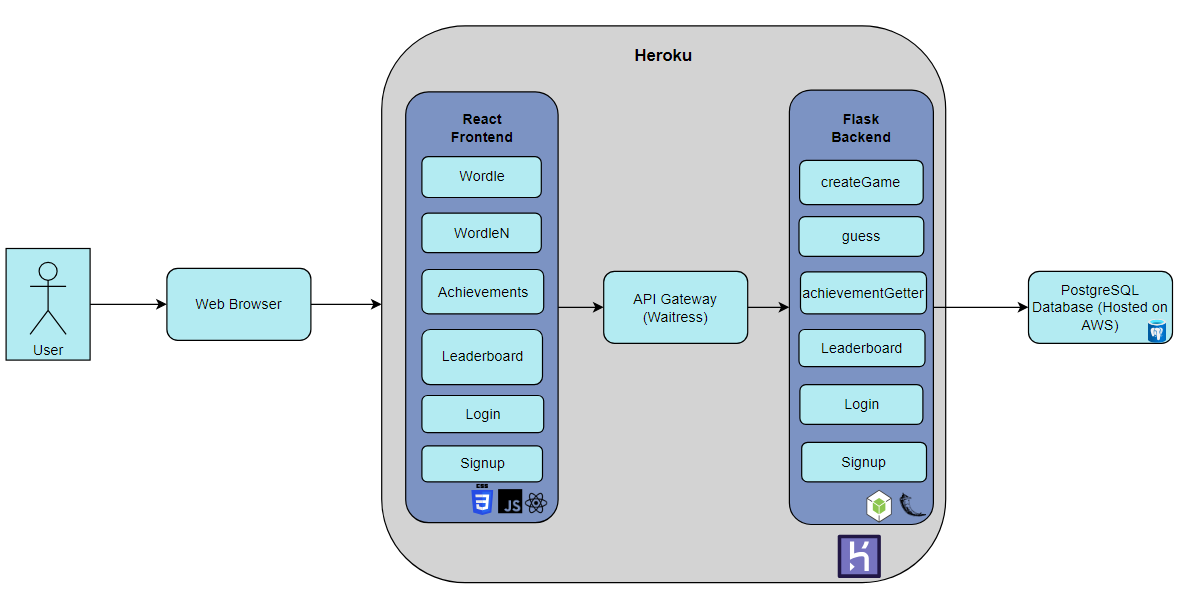
\includegraphics[width=\textwidth]{Architecture_Diagram_New_New.png
    } % Replace with your image file
    \caption{Architecture Diagram}
    \label{fig:example}
\end{figure}

The web application's front end uses React.js. After researching various front-end frameworks, the component-based architecture of React emerged as a natural choice, particularly for implementing keyboard functionality. This approach seemed well-suited for the different use cases anticipated for the keyboard, mainly because potential users had discussed the idea of an extended Wordle version.
Another significant consideration was React's status as one of the most widely used front-end frameworks in modern web development. The popularity of React presented an opportunity to enhance skills in web development beyond the scope of what was covered in the course. Additionally, React was chosen to facilitate learning and development in CSS, offering a chance to improve front-end development capabilities beyond creating websites with a Flask backend, using HTML and CSS with Bootstrap. Although these tools might have achieved a similar aesthetic outcome, the goal was also to expand expertise in front-end technologies.
A different framework was considered for the application's backend. However, after conducting research, it was determined that switching to Django would not offer enough challenges to significantly contribute to personal growth and development. Conversely, transitioning to an entirely different programming language was deemed too daunting, especially when concurrently learning JavaScript, React, and CSS.
The website's planned design also required many database calls. The database would store guesses, answers, and user data, just to name a few. For this approach to web development, SQLAlchemy seemed appropriate. Using the ORM style of SQL calls gave the ability to interact with the database in a Pythonic manner and let the calls and insertion of data be weaved into the code, as almost every call to the backend required some call to the database.

\section{Database}
\begin{figure}[h] % 'h' means 'here' - places the figure where it's defined
    \centering
    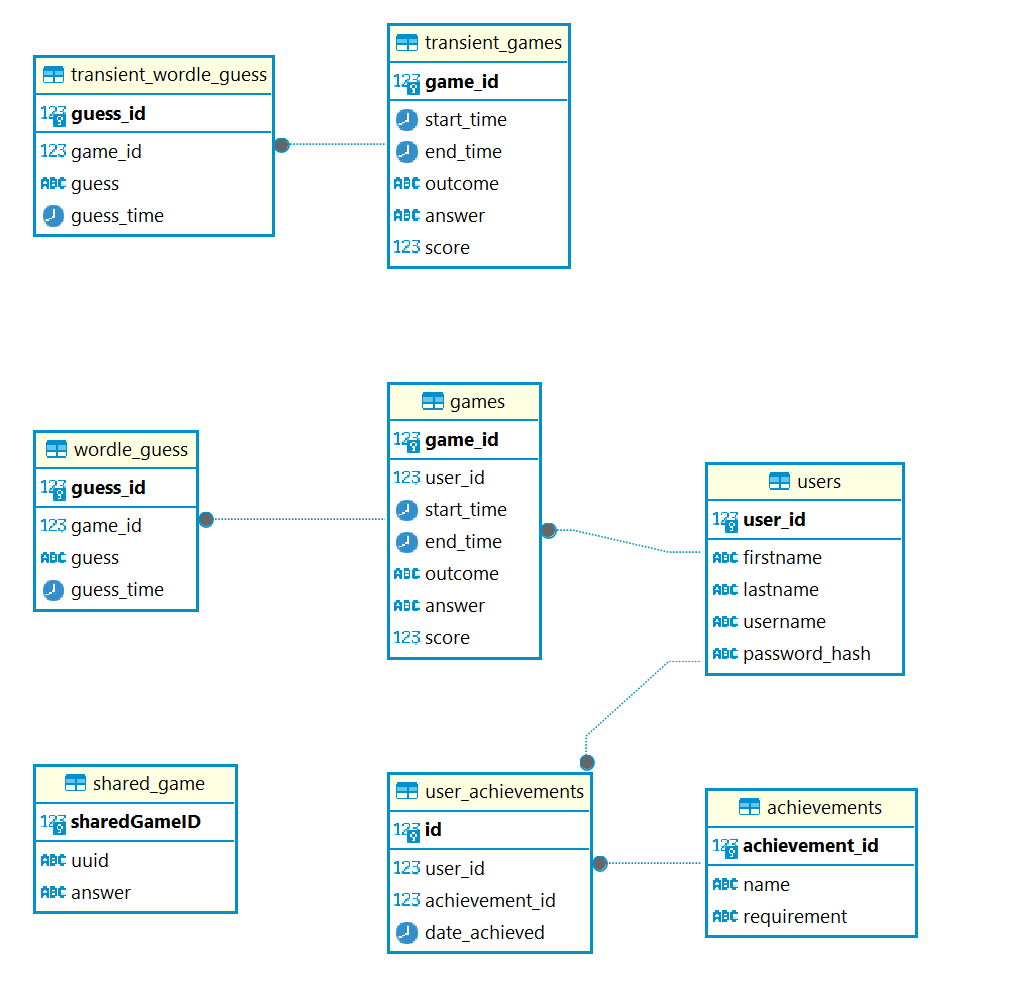
\includegraphics[width=\textwidth]{Database_Schema_Diagram.png} % Replace with your image file
    \caption{Database Schema Diagram}
    \label{fig:example}
\end{figure}
The database schema illustrates the system designed to handle both Wordle with no login and The Gauntlet
\subsection{Transient Mode (Wordle with no login)}
Two main tables are used in the transient mode: transientGames and transientWordleGuess.
\begin{itemize}
    \item transientGames
        \begin{itemize}
        \item gameId: A unique identifier for each game played.
        \item startTime and endTime: Timestamp fields that record when the game started and ended.
        \item Outcome: Stores the outcome of the game played.
        \item Answer: Stores the correct answer of the game.
        \item Score: Stores how well the user did in the game.
        \end{itemize}
    \item transientWordleGuess
        \begin{itemize}
        \item guessId: A unique id for each guess.
        \item gameId: A foreign key that links each guess to the corresponding game in the transientGames table.
        \item Guess: Stores the players guess.
        \item guessTime: Stores the time when the player guesses
        \end{itemize}
    \end{itemize}
    
\subsection{The Gauntlet}
\begin{itemize}
\item users
    \begin{itemize}
    \item userId: Primary key that identifies each user.
    \item firstName, lastName, username, passwordHash: All fields that store personal information of each user.
    \end{itemize}
\item games
    \begin{itemize}
    \item gameId: Primary key that identifies each user.
    \item userId: A foreign key which links the game to a specific user.
    \item startTime and endTime: Timestamps that indicate the time of the first guess and the time of the final guess.
    \item outcome: Stores the result of the game.
    \item answer: Stores the correct answer for the game.
    \item Score: stores the score achieved by the user.
    \end{itemize}
\item wordleGuess
    \begin{itemize}
    \item guessId: Primary key that identifies the guess.
    \item gameId: A foreign key that links the guess to the corresponding game in the games table.
    \item guess: stores the guess made by a user.
    \item guessTime: Timestamps when the guess was made.
    \end{itemize}
\item sharedGame
    \begin{itemize}
    \item sharedGameId: The primary key for instances of a shared game.
    \item uuid: Stores the unique identifier of each shared game.
    \item answer: The correct answer for the shared game.
    \end{itemize}
\item userAchievements
    \begin{itemize}
    \item id: The primary key for the user achievements table.
    \item userId: The foreign key that links achievements to a specific user.
    \item achievementId: A foreign key that links to a specific achievement on the achievement table.
    \item dateAchieved: The date when the achievement was earned by the user.
    \end{itemize}
\item achievements
    \begin{itemize}
    \item achievementId: The primary key for the achievements table.
    \item name: The name of the achievement
    \item requirement: The criteria that needs to be met to earn the achievement.
    \end{itemize}
\end{itemize}

\section{Unit Testing}
In this project, unit tests were implemented for key components across both the front end and back end. The backend unit tests were written using the unittest framework in Python, focusing on the application's core logic and APIs, such as the Wordle game logic and user authentication mechanisms. For example, the TestParseResult class in testServer.py contains several test cases that verify the correctness of the parseResult function, ensuring that it accurately evaluates the user's guesses against the correct Wordle answer.

\begin{lstlisting}[style=python, caption={The parseResult functions unit tests}]
class TestParseResult(unittest.TestCase):
    def test_all_correct(self):
        guess = "apple"
        answer = "apple"
        expected_result = ['correct', 'correct', 'correct', 'correct', 'correct']
        self.assertEqual(parseResult(guess, answer), expected_result)

    def test_some_present(self):
        guess = "apple"
        answer = "apply"
        expected_result = ['correct', 'correct', 'correct', 'correct', 'absent']
        self.assertEqual(parseResult(guess, answer), expected_result)

    def test_some_absent(self):
        guess = "apple"
        answer = "quick"
        expected_result = ['absent', 'absent', 'absent', 'absent', 'absent']
        self.assertEqual(parseResult(guess, answer), expected_result)

    def test_mixed(self):
        guess = "apple"
        answer = "plead"
        expected_result = ['present', 'present', 'absent', 'present', 'present']
        self.assertEqual(parseResult(guess, answer), expected_result)
\end{lstlisting}

Similarly, the front end unit tests were implemented using the @testing-library/react and jest frameworks, ensuring that the React components behave as expected under various conditions. Components such as Leaderboard, Achievements, and Wordle were tested. For instance, the Achievements.test.js file includes tests that simulate user interactions and validate that achievements are correctly fetched and displayed based on the user's progress. These tests help ensure that the front end functions correctly in isolation and integrates smoothly with the backend services.

\begin{lstlisting}[style=python, caption={Achievement frontend unit testing}]
describe('Achievements Component', () => {
    const mockUser = { token: 'mock-token' };
    beforeEach(() => {
        global.fetch = jest.fn();
    });
    afterEach(() => {
        jest.resetAllMocks();
    });
    it('fetches and displays achievements', async () => {
        const mockUserAchievements = ['Achievement 1'];
        const mockAllAchievements = ['Achievement 1', 'Achievement 2'];
        fetch.mockImplementationOnce(() =>
            Promise.resolve({
                ok: true,
                json: () => Promise.resolve(mockUserAchievements),
            })
        );
        fetch.mockImplementationOnce(() =>
            Promise.resolve({
                ok: true,
                json: () => Promise.resolve(mockAllAchievements),
            })
        );
        await act(async () => {
            render(<Achievement user={mockUser} />);
        });
        await waitFor(() => {
            expect(screen.getByText('Achievement 1')).toBeInTheDocument();
            expect(screen.getByText('Achievement 2')).toHaveClass('not-achieved');
        });
    });
    it('logs missing token', () => {
        const mockUserWithoutToken = {};
        console.log = jest.fn();
        render(<Achievement user={mockUserWithoutToken} />);
        expect(console.log).toHaveBeenCalledWith('No token available');
    });
});
\end{lstlisting}

\section{Components}
\subsection{App Structure}
\begin{lstlisting}[style=python, caption={The router function for the app structure}]
<Routes>
{!!(user.username) && <>
    <Route path="/wordle" element={<Wordle user={user} />} />
    <Route path="/achievements" element={<Achievements user={user} />} />
    <Route path="/leaderboard" element={<Leaderboard user={user} />} />
    <Route path="/wordleN" element={<WordleN user={user} setWordLength={setWordLength} wordLength={wordLength} uuid = {query}/>} />
    <Route path="/shared/*" element={<Wordle user={user} />} />
    <Route path="/sharedn/*" element={<Navigate to={"/wordleN"} />} />
</>}
{!(user.username) && <>
    <Route path="/signup" element={<Signup user={user} />}/>
    <Route path="/login" element={<Login user={user} setUser={setUser}/>}/>
    <Route path="/leaderboard" element={<Leaderboard user={user} />} />
</>}
<Route path="*" element={<Navigate user={user} to={!!(user.username) ? "/wordle": "/login"}/>} /> 
</Routes>
\end{lstlisting}
The App.js file handles the app structure. It is primarily a set of router fragments that link to each primary component of the web application. Because the user is being tracked on a leaderboard, we only want users to reach the Wordle component if logged in. The solution is that the useState is created inside the app file, and if a user is not currently logged in, they only have access to signup, login, and leaderboard. This is done using ternary operators, which only run the router fragment if the user has been validated. Instead, you will reach the final router fragment, which, depending on whether you are logged in, will route you to Wordle or the login page. 

\subsection{JWT}
\begin{figure}[h] % 'h' means 'here' - places the figure where it's defined
    \centering
    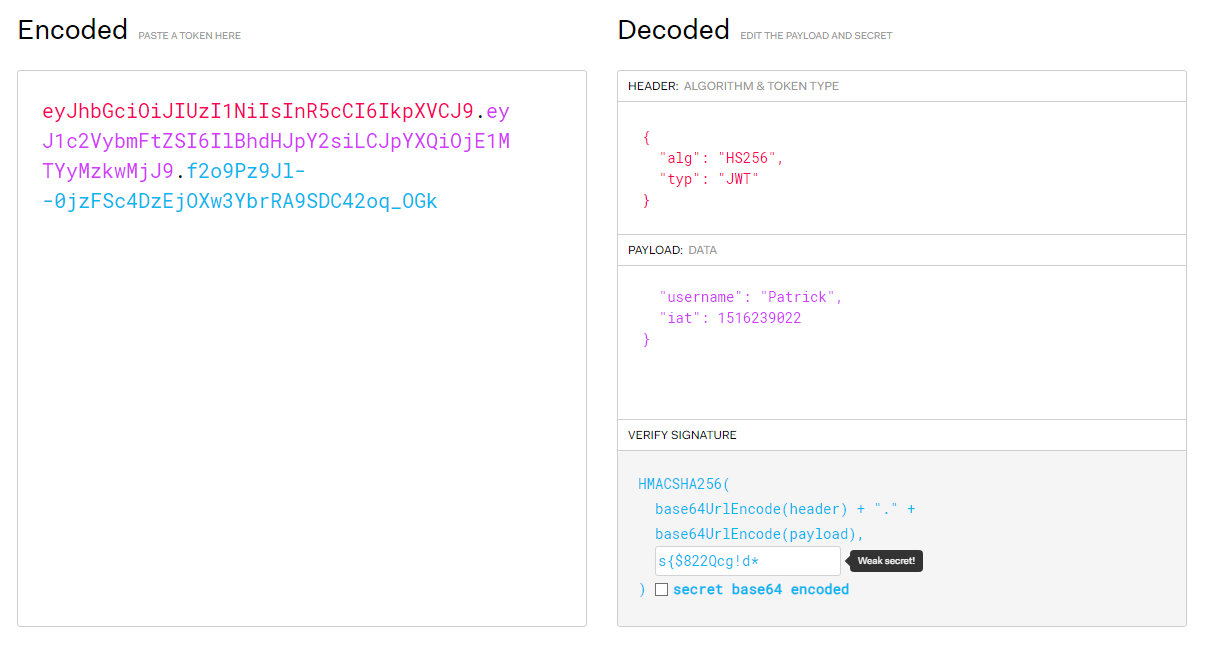
\includegraphics[width=\textwidth]{JWT_Decode.png} % Replace with your image file
    \caption{An example of a decoded JWT}
    \label{fig:example}
\end{figure}
When creating the Wordle app, it became apparent that there would need to be some sort of verification between the front and back end that the user that was set into the user UseState was the actual user logged in. After some research, Java Web Tokens were implemented into the website. With this, the payload would be the username encoded using a public/private key pair and stored in the user's local storage. Whenever a backend function call is made, the JWT is sent to the headers and decoded in the back end to verify the correct user. The username is then pulled from the JWT and used in many function calls to draw the correct user from the database.

\subsection{Keyboard}
During the early stages of the web app, when only the game's logic was in place, it became clear how vital the keyboard was to the “game feel” of Wordle. The keyboard not only gives users the ability to type in their guesses but also helps them keep track of the game's current state. When users have an idea for their next guess, they refer to the keyboard to see which one they have already tried. Without the keyboard, a user has to refer back to their guesses, which is frustrating and challenging to keep track of. 
The keyboard is relatively simple to implement. It passes information into a critical component, such as the letter it should submit, into the input box. It also passes the state of the key to the element, so the colour is updated for each guess. 

\subsection{WordleN}
\begin{lstlisting}[style=python, caption={The setWordLength handler function}]
const handleSetWordLength = (length) => {
        console.log("Setting Word Length " + length)
        setWordLength(parseInt(length));
        setDisabled2(true);
        setShowKeyboard(true);
        createGame(length)
        console.log('Word Length Set')
      };
    const backspace = () => {
        setGuess(guess.slice(0, -1))
    }
\end{lstlisting}
WordleN is a part of the efforts to increase the functionality of the Wordle application. In this component, the user can set a different word length of six, seven, or eight-letter words to increase the level of challenge. The logic is, of course, very similar to the main Wordle component. However, during personal testing in the production phase, it became clear that six guesses to find the solution of an eight-letter word would require more work for users. The solution is that you get an extra guess with each additional letter you must guess, meaning that eight-letter words give you nine guesses. Fortunately, the already implemented code for Wordle accounted for this and will still display guesses until the loss useState is updated. 

\subsection{Navbar}
A navbar is implemented on each application webpage for ease of use. This also uses the router function. The main challenges faced when implementing the navbar were only showing links to the pages that the user had access to and having an active breadcrumb to show which page was currently active. 
The solution to the first issue was very similar to what is done in the app structure. The Navbar also uses ternary operators based on whether the user is logged in. Even if the navbar still displayed the links to other application pages, users would be redirected if they weren’t logged in. However, for clarity’s sake, it is critical to display to the user the parts they can use depending on whether they are logged in. 
The answer to creating a breadcrumb is using the useLocation library provided by React. Each time the component mounts, a LocationProvider constant is created and passed to the navbar. A CSS class then adjusts the button's colour depending on the location.

\subsection{Wordle Frontend}
\begin{lstlisting}[style=python, caption={The loop that updates the results when they are received so they can be placed in the JSX}]
setResult(data.map(previousGuess => {
    let tempData = {
    }
    for (let i = 0; i < 5; i++) {
            let currentLetter = previousGuess.guess.charAt(i).toUpperCase()
            console.log(currentLetter)
            tempData["l"+ i] = {"letter": currentLetter,"result": previousGuess.result[i]}
            console.log(tempData)
            setKeyDictionary(keyDictionary.map(entry => {
                if (entry.key.toUpperCase() === currentLetter){
                    entry.state = previousGuess.result[i]
                }
                console.log(entry)
                return entry
            }))
    }
\end{lstlisting}
When the Wordle component mounts, a useEffect requests the backend to create a game for the user. This call will show no visual change to the component if the user is not in a game. Instead, it will just provide the new game ID within the database. If the user has a game currently active, the frontend will receive the user's previous guesses for that game with the correct labelling if the letter is either “correct”, “present”, or “absent”. This will then be displayed in the JSX as a table with the current guesses and the correct colour to indicate the state of the game. The colouring is done using CSS classes indicated to the front end, depending on what the dictionary returns each letter as.
When a user makes a guess inside the text box, the backend is requested to indicate the updated state of the game. This, in turn, updates the JSX displayed on the page by adding another row to the table with their guess printed out and colouring for each letter, indicating what state the letter is in.
When a user has reached a finished state in the game, whether they have won or not, a modal box is displayed asking if they wish to play again. If they do, the page doesn’t reload; instead, it resets all the useStates within the react component and clears the table of guesses. This modal box also allows users to share the word that they have just tried to guess and send it to another user. 

\subsection{Wordle Backend}
\begin{lstlisting}[style=python, caption={The parseResult function}]
def parseResult(guess, answer):
    confirmed_correct = [''] * len(answer)
    result = []
    letterCount = {}

    for i in range(len(guess)):
        if guess[i] == answer[i]:
            confirmed_correct[i] = guess[i]

    for letter in answer:
        letterCount[letter] = letterCount.get(letter, 0) + 1

    for i, letter in enumerate(confirmed_correct):
        if letter:
            letterCount[letter] -= 1

    for i in range(len(guess)):
        if guess[i] == answer[i]:
            result.append('correct')
        elif guess[i] in answer and letterCount[guess[i]] > 0:
            result.append('present')
            letterCount[guess[i]] -= 1 
        else:
            result.append('absent')

    return result
\end{lstlisting}
The backend will only create a game for the user if they still need to get it in the database with no outcome. In this case, the function creates an entry into the game table of the database with a random answer from the list of words of the correct length and the time the game started. The function returns the gameID to the front end to handle the guess function when the user submits their first guess. Because the leaderboard is tracking a user's average score, it is not appropriate for them to be able to refresh and immediately have a new game. If that were the case, then when the user got to five guesses, they could decide that they don’t believe they can achieve the correct answer, so they could refresh and try again with a new word. The solution to this is to check if they already have a game running without a result in the outcome column of the database. If the user does have a game when the createGame function is called, it is caught, and the backend will return a list of their current guesses, which, in turn, will map their guesses to a table and display it in the front. However, you cannot only send the guesses to the backend as then the words would not have the correct colouring to show whether the letter is in the correct position if it is in the word but not in the correct location, or if the letter is not in the word at all. This is why the parse result function is called in the dictionary and is returned as a JSON object.

How each letter is assigned one of the values, “correct”, “absent”, or “present”, is via the parseResult function. During the initial development of the Wordle component, the parseResult function was relatively simple. The function iterated through each letter of the guessed word, comparing it to the corresponding letter in the correct answer. If the letter in the guess matched the letter at the same position in the answer, it would add "correct" to the result dictionary for that letter. If the letter from the guess was present in the answer but in a different position, it would add "present" to the result dictionary. Otherwise, if the letter were not in the answer, it would be appended as "absent" in the result dictionary. This solution was somewhat functional; however, when put into users' hands, many complained about how letters were marked “present”.
In the original Wordle, if a letter has already been put into the correct position, there was no more of that letter. Suppose the user puts the letter into another position. In that case, it will mark it as “absent,” which created a challenge in creating parity with the original Wordle, which users criticised for making the game unnecessarily difficult. The solution to this was creating a dictionary that stored the number of times each letter was used and, when the letter was found, decreased the count of that letter by one. By doing this, if the letter count of that letter is more significant than zero, you can mark it as present. Otherwise, you mark it as absent.
When a user guesses the text box, a backend function is called, which returns a JSON object that returns each letter with a mark that denotes what colour to use for marking which letters in the word are in the correct position, present in the word but not in the proper position, or absent.
The win/loss state is also created using the backend. Each guess increments the guess count variable, which counts how many entries have been made into the Wordle Guess table with the current game's game ID. If that number reaches one more than the length of the word, giving you six guesses for a five-letter wordle, the game is counted as a loss within the database, and the time you lost is also logged. The function then calls the achievement checker function and rewards you accordingly. The guess function also checks whether the guess received from the front end is the same as the answer. In this case, the database will log the game as a win and the time you finished the game.

\subsection{Achievements Frontend}
The front end of achievements is a table formed from the two JSON objects returned from the backend. When the component is mounted, two separate backend calls are made. These backend calls are separate to pull a list of all the achievements, and then a call is made to send which achievements a user has received. It is then indexed in alphabetical order. The colour, which indicates whether you have received the achievement, is changed depending on which call the achievement came from. 

\subsection{Achievements Backend}
\begin{lstlisting}[style=python, caption={The achievementGetter function.}]
@app.route('/api/achievement_getter', methods=['GET'])
def achievement_getter():
    authoHeader = request.headers.get('authorization')
    print(authoHeader)
    token = authoHeader.split(" ")[1]
    try:
        decodedJwt = jwt.decode(token, "s{$822Qcg!d*", algorithms=["HS256"])
        user = User.query.filter_by(username=decodedJwt['username']).first()
        achievements = UserAchievement.query.filter_by(user_id=user.user_id).all()
        return jsonify ([achievement.achievement.name for achievement in achievements])
    except:
        print(traceback.format_exc())
        return jsonify({"error": "Invalid token"}), 400
\end{lstlisting}
The functionality for achievements in the back end is split into three different functions: one for checking achievements that are called when an outcome is decided for each game, another for sending the user's current achievements to the front end, and one for sending a complete list of achievements to the front end. The latter two are calls made in SQLAlchemy. The first is searching for all the achievements listed in the UserAchievement table matched on the userID fed to the function. The second searches for a complete list of achievement names in the achievements table. 
The achievement checker is more complex as the achievements must be checked differently. We first have to check the user's total wins and losses, both done through calls to SQLAlchemy. Then, the function checks the score of the current game and the time that has been fed to the function. It also tracks averages and creates the game time by removing the end time from the start time. This information is then used to loop through the list of achievements and check whether the user has achieved the achievements with basic logic operators. If the user has completed the achievement and has yet to test it in the User Achievement table, it is appended to a list that is returned when the function is finished. The function then bulk saves the objects added to userAchievements and returns the list. 

\subsection{Leaderboard Frontend}
The leaderboards are returned from the backend and almost fully formed inside the JSON object. These backend calls are stored in a useEffect so that the server will be called as soon as the component mounts. The data is stored in separate useStates when returned from the backend and mapped into JSX elements to be displayed to the user. 

\subsection{Leaderboard Backend}
\begin{lstlisting}[style=python, caption={The Leaderboard SQL call}]
WITH scored_games AS (
    SELECT g.game_id, g.user_id, COUNT(1) AS score, g.start_time, g.end_time
    FROM games g 
    INNER JOIN wordle_guess w ON w.game_id = g.game_id
    WHERE g.outcome IS NOT NULL
      AND LENGTH(g.answer) = 5
    GROUP BY g.game_id, g.user_id, g.start_time, g.end_time
)
SELECT u.firstname,
       ROUND(AVG(g.score), 2) AS score,
       ROUND(AVG(EXTRACT(EPOCH FROM g.end_time) - EXTRACT(EPOCH FROM g.start_time)), 2) AS avg_time,
       RANK() OVER (
           ORDER BY ROUND(AVG(g.score), 2) ASC, 
                    ROUND(AVG(EXTRACT(EPOCH FROM g.end_time) - EXTRACT(EPOCH FROM g.start_time)), 2) ASC
       ) AS rank
FROM users u
INNER JOIN scored_games g ON u.user_id = g.user_id
GROUP BY u.firstname
ORDER BY score, avg_time;
\end{lstlisting}
The leaderboards are created through an SQL query that joins Wordle Guess and the games table. The call then tracks the average score from all users' games and figures out the average length of time a Wordle game takes them. This table is then joined to the user's table from the userID and grouped by the user's first name. It is then ordered by score, and if there is a tie-in score, it is decided by the average time it takes them to complete a Wordle. All the back end does for this is execute the query and return it to the front end in the JSON object. It has to call this query multiple times, with the only adjustment being the length of the answer. This is done so there can be separate leaderboards for each length of Wordle word that can be played. 

\subsection{Share Frontend}
\begin{lstlisting}[style=python, caption={The Share call used on click}]
const share = async () => {
    try {
        const response = await fetch('/api/createSharedGame', {
            method: 'POST',
            headers: {'Content-Type': 'application/json'},
            body: JSON.stringify({ answer: answer})
        })
        if (response.ok) {
            const data = await response.json();
            navigator.clipboard.writeText(`${window.location.origin}/shared/${data.uuid}`)
            enqueueSnackbar('Link copied to clipboard')
        }
    }
    catch (error) {
        console.error(error)
    }
}
\end{lstlisting}
All that is done to accommodate share functionality is creating a route in a router fragment within the app structure. This will redirect to Wordle or WordleN, depending on which page you got the share link from. The modal box at the end of each game has a share button. When this is clicked, a request is sent to the backend, and with this, the frontend sends the answer. A uuid is then returned to the front end, and the body of the link is created when a user clicks on it.

\subsection{Share Backend}
The backend generates a uuid and creates a game in the SharedGame table in the database. All this table contains is a UUID and an answer. When this link is used, the uuid will be pulled from the link and checked against the SharedGame table. All that is done after this is the row with that uuid is found, and the answer is then sent to the createGame function. When a game is returned to the front end, it will function the same, but the answer will now be the word from the game that the user sent it from.

% !TEX root =  ../Dissertation.tex

\chapter{Evaluation}
\section{Surveys and User Satisfaction}
The findings of this project are predominantly split into two. Findings from evaluating users and findings from the data tracking done on the website by Google Analytics. This section of the report will distil the findings of these two methodologies and what can be learned from the twenty users who used both applications, Wordle with no login and Wordle with increased features, to track how many more were retained from the increased features. 

Before users entered the experiment, an entrance survey was sent to gather information about their previous interactions with Wordle. The amount that people have played and still play varied greatly. The entrance survey clearly showed that most felt positive about adding more features and more of an ability to interact with friends and family. There was a clear consensus that adding the features suggested on the goals page was a great starting point to add more intractability to a daily game genre web app. 

In the exit survey, most users were satisfied with the gauntlet overall, with an average rating of 4.2/5. The leaderboard feature was the clear favourite for user satisfaction, achieving a rating of 4.73/5. From the comments, it is evident that it did elicit the hoped effect from users. 14/15 users said that the leaderboard encouraged them to play more, and 11/15 users mentioned the word "competition" or "competitiveness; the rest praised the feature for its social aspects.

Something else that became clear was that many users did not understand or enjoy the share feature, with it achieving a rating of 3.67/5. When checking the database, it was the least-used feature in the web application as it was only used for twelve different words over the seven days. Because of this, a question was added to the exit survey asking users if they understood what the share button did. 33 percent of people did not understand the feature and quite a few of the users who did were not in favour of it. What emerged from the exit form was that many people didn't explore the feature. One user commented that "there was no incentive to share". In hindsight, what could have been done for this is associating achievements with shared games; this would be similar to how Clash of Clans have incentives to invite other users to use the game, which would help with user acquisition. While the share feature was not a complete failure, some users still used and enjoyed it. It has become evident that there was not enough clarity as to what the share function did, and there was not much to be gained in using it. 

Achievements did well in satisfaction, not as well as leaderboards but not as poorly as shared. It ended with an average score of 4/5 from users. 27 percent of users said they were not encouraged to continue playing because of the achievements system. Originally when produced the main issue that was foreseen with achievements was the rudimentary nature of them. None of them were too in-depth and primarily based on how many wins and losses you achieved. What most users took issue with, however, was that there was no social aspect to them. One user mentioned, "I personally had no interest in obtaining achievements for the game. The ones I did get were mostly by luck/accidentally. It was not a negative to my experience. Perhaps if there were a leaderboard (or other way of comparing to others) for the achievements themselves this would be different (if there was, I didn't notice it).". Another user said, "I like when achievements are part of a bigger network like Steam or Xbox but they don't motivate me as a one-off.". From these comments, a change that could be made that would improve the achievement system could be the ability to compare your achievements to another user, similar to how you can on Steam, adding a level of sociability not yet found in the achievements system. 

\begin{figure}[h] % 'h' means 'here' - places the figure where it's defined
    \centering
    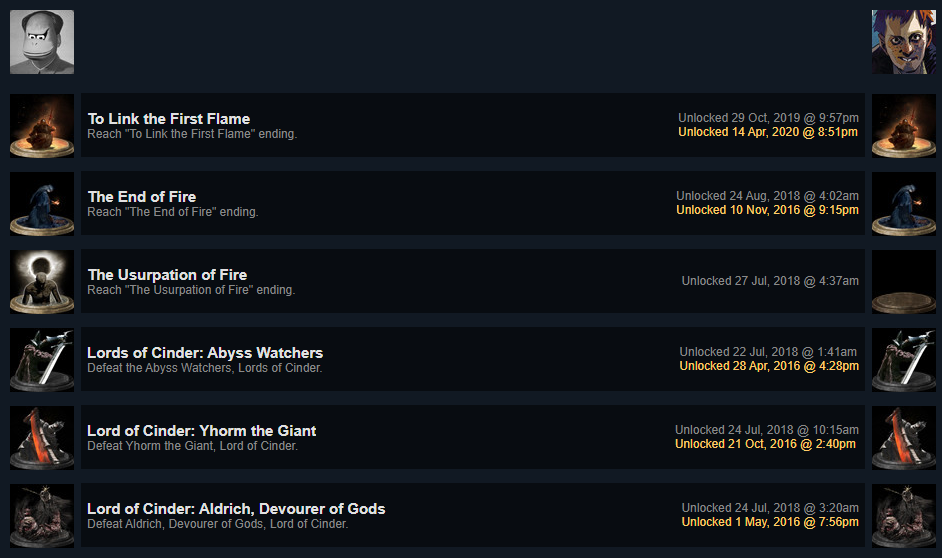
\includegraphics[width=\textwidth]{Steam_Achievements_Comparison.png} % Replace with your image file
    \caption{An example of comparing achievements on Steam}
    \label{fig:example}
\end{figure}

Wordle with increased word length also seemed to be a success for user satisfaction with 27 percent of players listing it as the number one feature that encouraged them to play more. One concern when developing this feature was that it would be too frustrating for users to play, as coming up with an eight-letter word is significantly harder than a five-letter word. In the exit survey, most commented that while it was fairly challenging, the users also felt more rewarded when they solved it. One user commented, "Increased word length up to 6 was challenging, but the number of eliminated letters per guess makes 7 and 8 letters quite easy". This was a surprise, but perhaps only one user commenting on this makes it a partial outlier in the game's believed increased difficulty. 

\section{Data Analytics}
All users had access to both websites and were prompted to use them as much as they pleased for a week. Google Analytics was set up for both websites to compare how many users remained using both websites. This allows other valuable information to be gleaned from the analytics that Google provides. 

As expected, Wordle had no features, and The Gauntlet had roughly the same number of users, with the Gauntlet at 34 and Wordle at 33 over the seven days. While the website was only sent to twenty people, it's apparent that some users sent the website to others, so it is not unexpected that there are a few more users. Interestingly, on the first day of the experiment, two more users used Wordle over the Gauntlet. 

\begin{figure}[h] % 'h' means 'here' - places the figure where it's defined
    \centering
    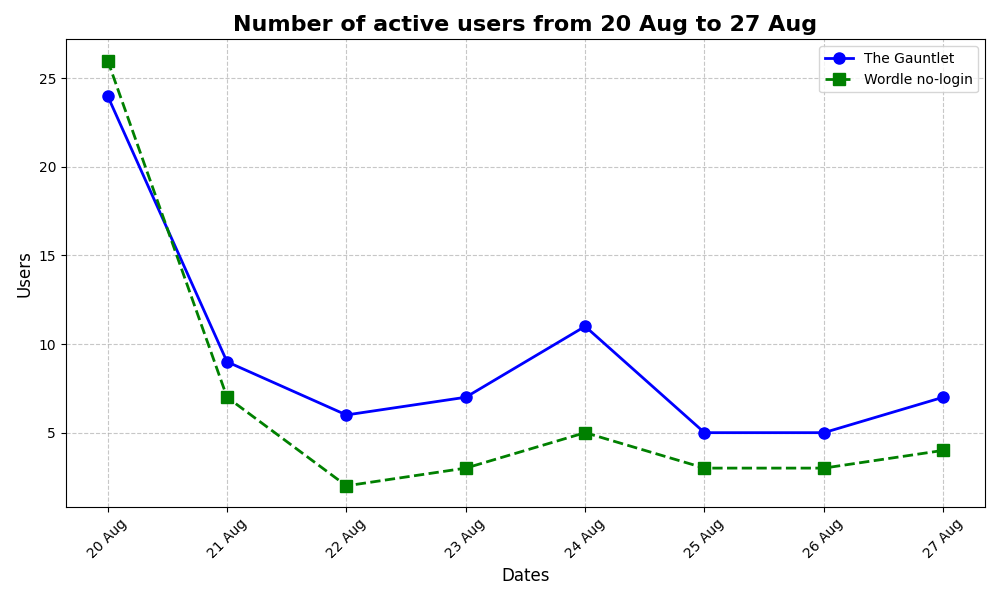
\includegraphics[width=\textwidth]{Number of Active Users Gauntlet.png} % Replace with your image file
    \caption{Graph of active users during the experiment on both web apps}
    \label{fig:example}
\end{figure}

After the first day, usage sharply declines. This is expected with games such as this, as shown by Mistplay, a company that focuses on a loyalty reward system for gamers using its suite of games. Mistplay released an article showing the retention rates of its games, and even on the first day, it retains only 30 percent of the users who try the application\cite{mistplay2024}. On the third day, The Gauntlet's user numbers stabilised, maintaining a user base of five to seven users daily, with an uptick on Saturday to eleven users. Wordle, by comparison, on the third day, had stabilised to a user base of two to four, with an uptick on Saturday of a user base of five. These increases during the weekend are likely due to users playing more games on a weekend rather than a weekday (Cite article here). From this data, it is apparent that the users have tended more to use The Gauntlet over Wordle with no login in terms of active users each day.

Another aspect in which The Gauntlet has outperformed Wordle with no login web app is user engagement. Over the seven days that the experiment lasted, Wordle, with no login, had an average engagement time of 1 minute and 44 seconds. Conversely, The Gauntlet had an average engagement time of 10 minutes and 54 seconds. A part of this increase can likely be accredited to users having to spend longer to solve a longer. Also, users will be more likely to play multiple games in a single session to improve their leaderboard rating or attempt to attain an achievement. 

\begin{figure}[h] % 'h' means 'here' - places the figure where it's defined
    \centering
    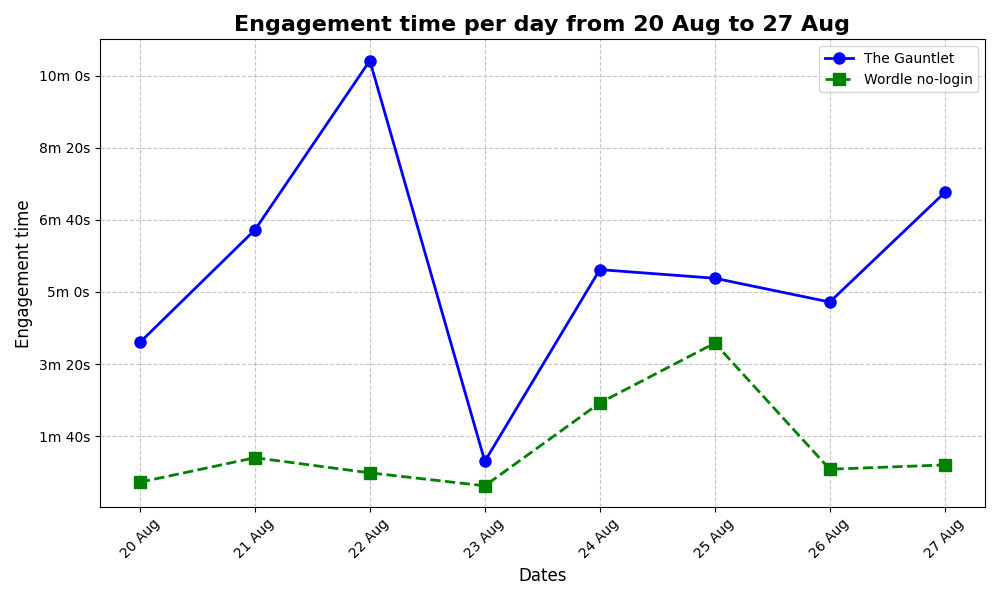
\includegraphics[width=\textwidth]{Engagement_Time.png} % Replace with your image file
    \caption{Average Engagement time each day for both web apps}
    \label{fig:example}
\end{figure}

\clearpage

Google Analytics also tracks the number of "events" triggered on a website. An "event" occurs whenever a user interacts with the website in any way, whether they change pages, make a guess, or change the website's state. Throughout the experiment, Google Analytics tracked 304 events on the Wordle without login, while The Gauntlet had 1500. It should be pointed out that this may not be the strongest comparison between the two websites, as The Gauntlet has many more events to trigger over Wordle with no login. Looking at the database for overall games, 191 games were played on The Gauntlet, while only 40 games were played on Wordle with no login. 

\begin{figure}[h] % 'h' means 'here' - places the figure where it's defined
    \centering
    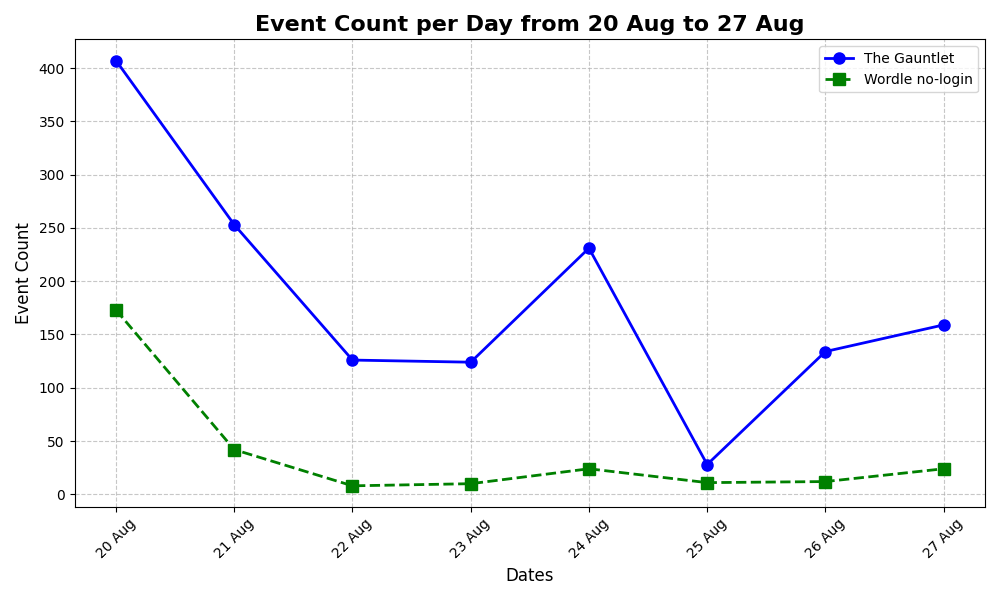
\includegraphics[width=\textwidth]{Event_count_per_day.png} % Replace with your image file
    \caption{Event Count each day for both web apps}
    \label{fig:example}
\end{figure}

Overall, it is clear that The Gauntlet has better metrics in every aspect compared to Wordle with no login. While it is hard to show in the data what aspects of The Gauntlet increased user retention the most, a general idea can be formed by the user satisfaction as user satisfaction is shown to be a direct indicator of user retention in features (Cite StumbleUpon article). The share feature seems to have had little effect due to unclear signposting of what the feature did and users not thinking it added much value to the overall web app, while leaderboards seem to be the retention technique with the greatest effect, achievements also being a valuable addition to retention.
\clearpage
\section{Requirements Met}
Now that The Gauntlet has been tested and evaluated by users and data metrics, it's pertinent that the functional and non-functional requirements are checked to see if it has reached its desired state. Most requirements are met, so this section will look at those that weren't.

\begin{figure}[h] % 'h' means 'here' - places the figure where it's defined
    \centering
    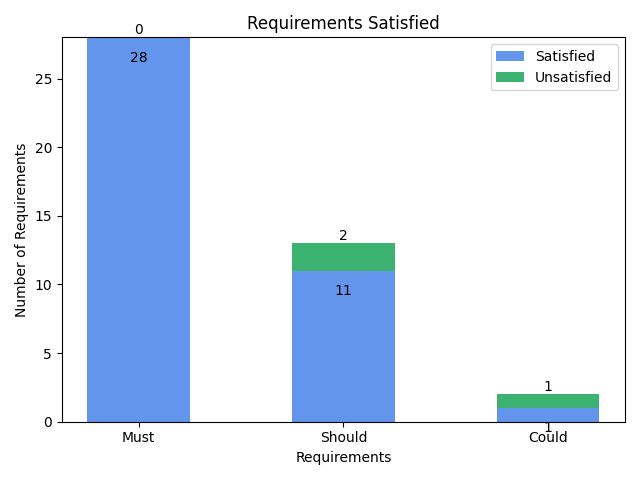
\includegraphics[width=\textwidth]{Requirements_Met.png} % Replace with your image file
    \caption{Graph of requirements met.}
    \label{fig:example}
\end{figure}


\begin{itemize}[leftmargin=*, label=\textbullet]
    \item \textbf{Have an option to suggest achievements} This was originally conceptualised as an offering so that users could suggest achievements in a submission box to better understand how the achievement section could be improved. When prototyping this component, it harmed the aesthetics of the achievements page greatly for something no longer believed to add too much value to the project, as users were generally messaging the developer personally to suggest changes about all aspects of the website. In the future, something like this could be added as a separate page to invite suggestions on changes to any part of the website, as personal messages about improving the site to the developer directly are not scalable enough to consider all users' opinions.

    \item \textbf{Layout should match the qwerty layout} This functional requirement was only attempted later in development when dealing with fixes and smaller additions. When attempting to add this requirement, it created large issues on the phone version of the web application where the keyboard would take up an amount of the screen, which meant users could not fully see the game they were playing. In future works, it should be possible to achieve this requirement, and this functionality was just left unfixed due to time constraints.

    \item \textbf{Have guesses be checked against a comprehensive English dictionary}
    During the development of the web application, many different large libraries of English words were used to check that users' words were valid guesses for Wordle. The issue that was raised by users when they eventually started using the web application was that these libraries invalidated words that should be validated. Eventually, this feature was scrapped to prevent users from being frustrated with invalid guesses. There must be a library large enough to fix this issue, but one that had open access was not found during development. 


\end{itemize}
% !TEX root =  ../Dissertation.tex

\chapter{Discussion}

\section{Limitations and Lessons}
There are an endless number of editions and changes that the web application would have received if there had been no time constraints. That being said, a few in particular should be mentioned that would have had a significant impact.
Firstly, if development had been finished sooner, users could have used the application longer, giving more reliable data. Not only would the data have given readers a better idea about the long-term effect of these features, but users would have had more time to give feedback that could have been considered when making another round of changes. 
One of the changes immediately requested that should have been taken into account was to ensure the application could be used on the phone. When the web application was first sent out, if it was loaded on a smaller screen, it would only display the keyboard, and the entire interface would be unusable. This massive issue was fixed on the second day by adjusting the CSS for smaller screens. 
There were also accessibility issues when users used the web application on the phone. One potential participant had to drop out of the experiment as they could only use their phone during the week, and their visual impairment meant that they used large text when using their phone, which is a setting within many smartphones. This caused the text to appear fragmented on the page, and unfortunately, it couldn’t be fixed before the experiment ended. If development were to start again from scratch, it would have been approached with more mindfulness to accessibility for all users.
 Perhaps naively, the web application was only made with a desktop in mind, and as development had taken place on a 1440p screen, there was an assumption that it would still work on smaller devices. The issue was so prevalent because of all the pageviews on the site, 42 percent of which were visited on the phone. The fix that made the application usable on the phone also did not have the neatest layout and required scrolling to get to the submit word button, particularly on eight-letter wordles, where a user receives nine guesses. In the future, when making a game like this again, it would be more important that building the web application from the start with smaller screens in mind would lead to higher satisfaction with users.
Leaderboards also underwent an iteration when users started playing. Initially, only one leaderboard contained the data for all word lengths. It was quickly realised that this discouraged users from playing some of the longer word lengths, as these are harder to get in a small number of guesses. This was fixed quickly, but this may have discouraged people if they were not often checking the leaderboards. 
Another issue with the Leaderboards is that the tiebreaker for people with the same average score is their average time to complete a game. The average time is calculated by checking the end time of each game minus the start time of each game in seconds. Then, it was used as their average time. While this seemed logical at the time, something that hadn’t been considered was when a user leaves a game unfinished overnight. This led to very long average times that did not indicate how long a user takes to complete a game. 
Another issue that needed to be fixed by the end of development was invalidating guesses. A user can type any assortment of letters as a guess, and it will accept it as a word. This is because many word lists were tried during development but would not take some words as valid during testing. Some libraries needed the full range of answers you can get in the game. This led to issues where people had to ask for their game to be deleted from the database as they knew the correct word but could not use it as an answer. After many different libraries were tested, it was decided that it would be best to avoid having this guess checker to stop people from getting frustrated with actual words that are not considered valid.
 While this is a limitation to achieving parity with the original Wordle game, it led to users' creativity when trying to complete the more complex challenges that higher-length words provided. Users would throw away a guess to try and find where the vowels were in the eight-letter words, making it easier for them. This development of a ‘meta’ of how to complete higher-length wordles was an exciting example of the innovation users can find when the developer allows it. 
 
\section{Future Works}
Moving forward with the application, many additions could be made to improve it, making the experience more enjoyable. It would be interesting to develop new games from the application and make it less inspired by Wordle and instead NYTGames. NYTGames acquired Wordle a few months after its creation and added it to a similar set of verbal and non-verbal reasoning games. This includes Crosswords, Mini Crosswords, Wordle, a game called connections where you have to find the links between 16 words, a more complex word search and many others. Adding these many features would likely increase retention and allow users to pick which games they enjoy the most and only play those. In the original scope of this project, it was intended to have two more games, and it would be ideal to develop a few more so users can play Wordle. This would also allow us to know how much of a factor it was of people needing to be retained because they were bored of Wordle. 

To make the experiment have more compelling data with more usability, more retention techniques could be developed, and when an account is created, the user is set 3 retention techniques from a list of 10. With this, you could make more precise decisions about which strategies were most effective, and creators of web applications in the daily word game genre could make more accurate decisions on how to spend development time creating retention techniques that will retain users. 

\section{Threats to Validity}
While the data tracked on both websites indicate that the study has shown the hypothesis to be true based on user satisfaction and data metrics. It should be apparent that only tracking user retention for seven days could lead to misunderstandings about how well the web application would perform in the long term. From the first seven days, we can be fairly certain that The Gauntlet would outperform Wordle with no login, but how much and whether the Gauntlet would also lose its player base remains unclear. 
The small sample size of users may also raise questions about how well the website would have retained players if the web application had started with 1000 or more users. From the data of other games, it is clear that user retention would not remain steady, as it is expected that after thirty days, user retention will usually drop another 3-4 percent from the initial user base.\cite{mistplay2024}

\section{Conclusion}
The goal of developing both web applications was to explore how the implementation of retention strategies impacts user satisfaction, engagement, and retention. The data metrics and user surveys show that incorporating retention techniques into The Gauntlet led to significantly better performance compared to Wordle without a login system, particularly in terms of user satisfaction, engagement time, and user retention. Features such as leaderboards, achievements, and enhanced functionality played a key role in driving these improvements. However, there is still room for further exploration. Future work could focus on developing adaptive retention strategies tailored to individual users. This approach would allow developers to identify the most effective techniques for maximizing user satisfaction and retention on a more personalized level.


\bibliographystyle{abbrv}
\bibliography{bibliography}

\chapter{Appendices}
\section{Exploratory Survey}

\section*{Questionnaire}

\begin{enumerate}

    % Question 1
    \item \textbf{When was the last time you played Wordle?} \\
    Please select one option:
    \begin{itemize}
        \item I play every day
        \item I have played at least once in the last week
        \item I have played at least once in the last month
        \item I have played at least once in the last two months
        \item I have played at least once in the last six months
        \item I have played Wordle at least once since release
        \item I have never played Wordle
    \end{itemize}

    % Question 2
    \item \textbf{Which option best describes you?} \\
    Please select one option:
    \begin{itemize}
        \item I play Wordle daily.
        \item I used to play Wordle daily but now I play less frequently.
        \item I used to play Wordle daily but no longer play.
        \item I play Wordle occasionally.
        \item I used to play Wordle occasionally but have stopped.
        \item I have never played Wordle.
    \end{itemize}

    % Question 3
    \item \textbf{If you no longer play Wordle, could you please share the reasons why?} \\
    \textit{Enter your answer:} \underline{\hspace{10cm}}

    % Question 4
    \item \textbf{What could make you start playing Wordle again if you've stopped?} \\
    Please select one option:
    \begin{itemize}
        \item New features or updates
        \item More challenging puzzles
        \item Playing with friends/family
        \item I’m unlikely to start playing again
        \item Other: \underline{\hspace{5cm}}
    \end{itemize}

    % Question 5
    \item \textbf{How long would you typically spend on Wordle in a day?} \\
    Please select one option:
    \begin{itemize}
        \item Less than 5 minutes
        \item 5-10 minutes
        \item 10-20 minutes
        \item More than 20 minutes
        \item It varies depending on the difficulty
    \end{itemize}

    % Question 6
    \item \textbf{Would you be interested in additional Wordle content or variations?} \\
    Please select one option:
    \begin{itemize}
        \item Yes, I would like more variations
        \item No, I prefer the original game
        \item No, I’m not interested in variations
    \end{itemize}

    % Question 7
    \item \textbf{How happy are you with the current version of Wordle?} \\
    \textit{Please rate your satisfaction on a scale of 1 to 10 (1 = not happy at all, 10 = extremely happy):}
    \begin{itemize}
        \item 1
        \item 2
        \item 3
        \item 4
        \item 5
        \item 6
        \item 7
        \item 8
        \item 9
        \item 10
    \end{itemize}

\end{enumerate}

\section{Questionnaire Results}
\begin{figure}[h] % 'h' means 'here' - places the figure where it's defined
    \centering
    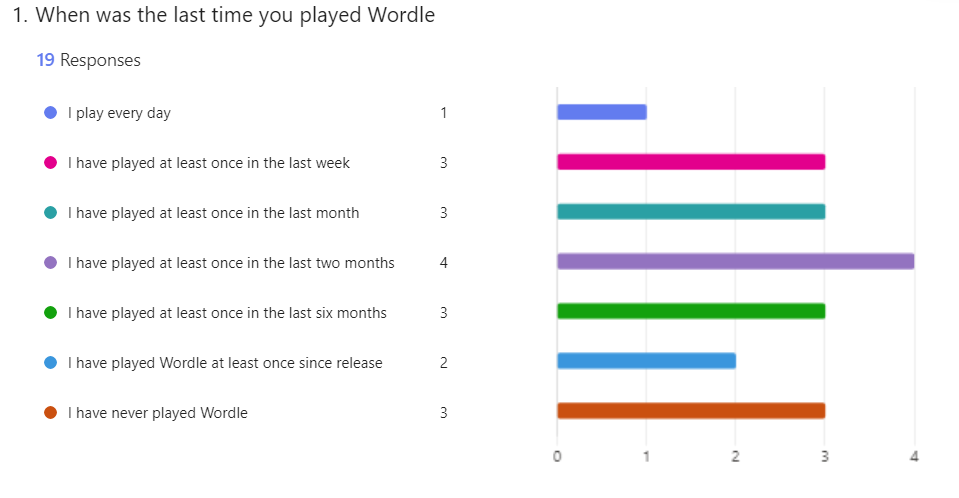
\includegraphics[width=\textwidth]{WordleResponse1.png} % Replace with your image file
    \label{fig:example}
\end{figure}
\begin{figure}[h] % 'h' means 'here' - places the figure where it's defined
    \centering
    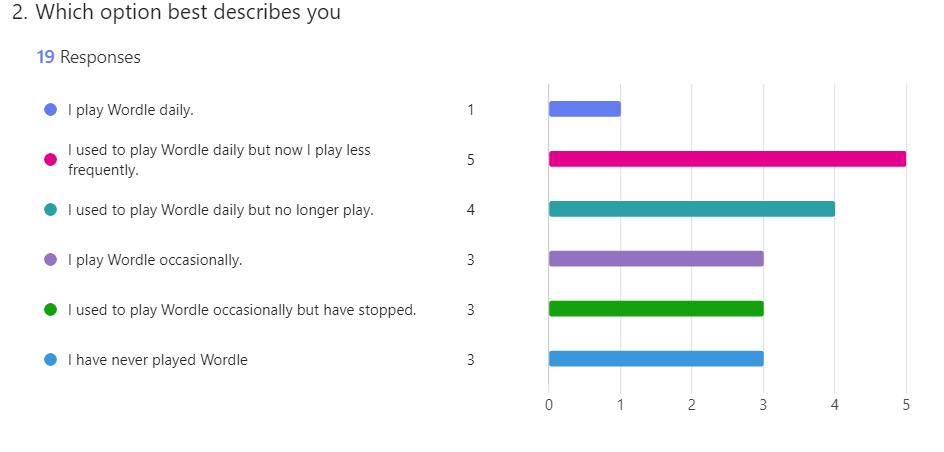
\includegraphics[width=\textwidth]{WordleResponse2.png} % Replace with your image file
    \label{fig:example}
\end{figure}
\begin{figure}[h] % 'h' means 'here' - places the figure where it's defined
    \centering
    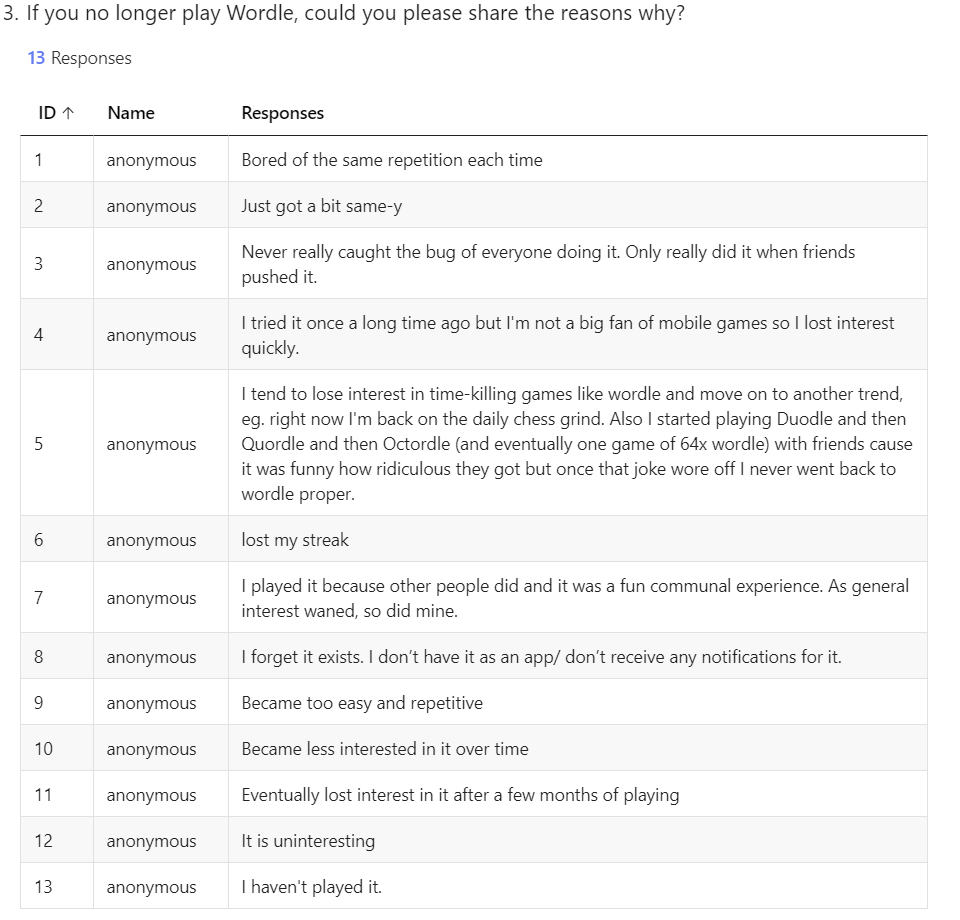
\includegraphics[width=\textwidth]{WordleResponse3.png} % Replace with your image file
    \label{fig:example}
\end{figure}
\begin{figure}[h] % 'h' means 'here' - places the figure where it's defined
    \centering
    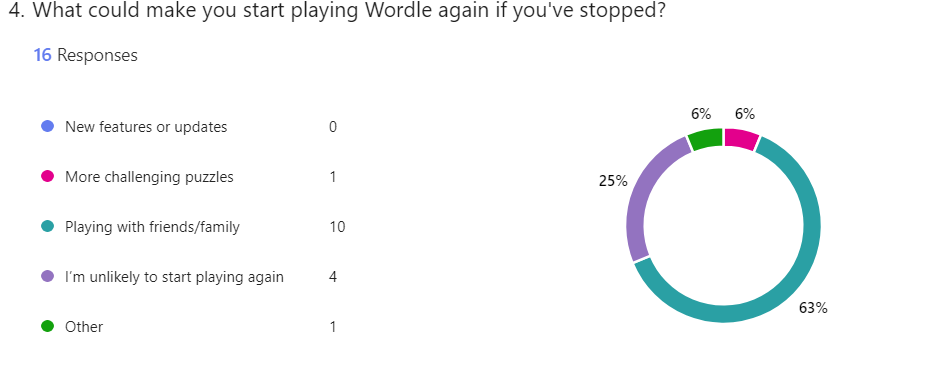
\includegraphics[width=\textwidth]{WordleResponse4.png} % Replace with your image file
    \label{fig:example}
\end{figure}
\begin{figure}[h] % 'h' means 'here' - places the figure where it's defined
    \centering
    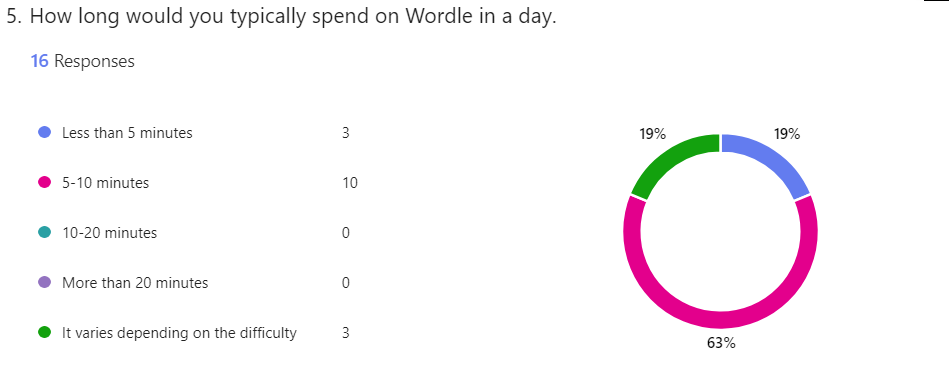
\includegraphics[width=\textwidth]{WordleResponse5.png} % Replace with your image file
    \label{fig:example}
\end{figure}
\begin{figure}[h] % 'h' means 'here' - places the figure where it's defined
    \centering
    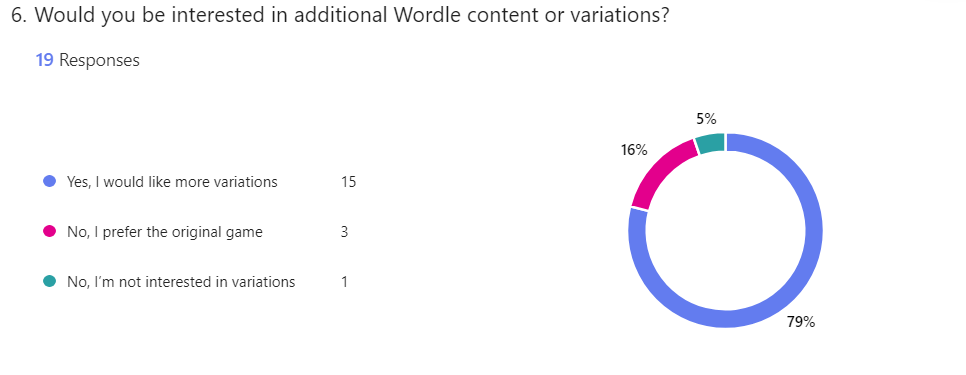
\includegraphics[width=\textwidth]{WordleResponse6.png} % Replace with your image file
    \label{fig:example}
\end{figure}
\begin{figure}[h] % 'h' means 'here' - places the figure where it's defined
    \centering
    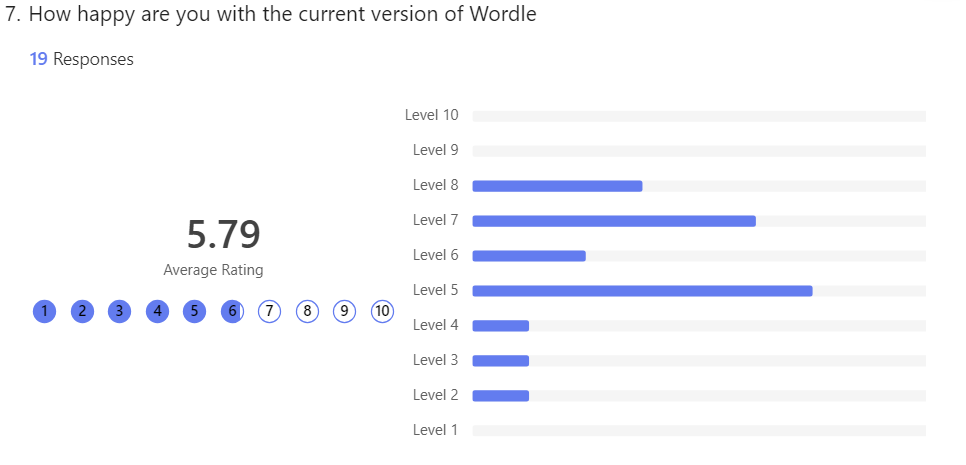
\includegraphics[width=\textwidth]{WordleResponse7.png} % Replace with your image file
    \label{fig:example}
\end{figure}
\clearpage
\section{The Gauntlet Exit Form}

\begin{enumerate}
    \item \textbf{What is your name?} \\
    \textit{(Enter your answer below.)}
    \vspace{2cm}
    \hrulefill
    
    \item \textbf{How much did you enjoy The Gauntlet (Wordle with more features)?} \\
    (On a scale of 1 to 5, with 1 being not enjoyable and 5 being very enjoyable.)
    \begin{enumerate}[label=(\arabic*)]
        \item 1
        \item 2
        \item 3
        \item 4
        \item 5
    \end{enumerate}

    \item \textbf{How much did you enjoy Wordle with increased word length?}
    \begin{enumerate}[label=(\arabic*)]
        \item 1
        \item 2
        \item 3
        \item 4
        \item 5
    \end{enumerate}

    \item \textbf{How frustrating did you find Wordle with increased word length?}
    \begin{enumerate}[label=(\arabic*)]
        \item 1
        \item 2
        \item 3
        \item 4
        \item 5
    \end{enumerate}

    \item \textbf{How much did you enjoy the Leaderboards feature?}
    \begin{enumerate}[label=(\arabic*)]
        \item 1
        \item 2
        \item 3
        \item 4
        \item 5
    \end{enumerate}

    \item \textbf{How much did you enjoy the achievements feature?}
    \begin{enumerate}[label=(\arabic*)]
        \item 1
        \item 2
        \item 3
        \item 4
        \item 5
    \end{enumerate}

    \item \textbf{How much did you enjoy the shared game feature?}
    \begin{enumerate}[label=(\arabic*)]
        \item 1
        \item 2
        \item 3
        \item 4
        \item 5
    \end{enumerate}

    \item \textbf{Do you believe the Leaderboard encouraged you to play more?}
    \begin{enumerate}[label=(\arabic*)]
        \item Yes
        \item No
    \end{enumerate}

    \item \textbf{Please explain why.}
    \vspace{2cm}
    \hrulefill

    \item \textbf{Do you believe the Achievement system encouraged you to play more?}
    \begin{enumerate}[label=(\arabic*)]
        \item Yes
        \item No
    \end{enumerate}

    \item \textbf{Please explain why.}
    \vspace{2cm}
    \hrulefill

    \item \textbf{Did the Shared game feature encourage you to play more?}
    \begin{enumerate}[label=(\arabic*)]
        \item Yes
        \item No
    \end{enumerate}

    \item \textbf{Please explain why.}
    \vspace{2cm}
    \hrulefill

    \item \textbf{Were you aware what the Share button did at the end of each game?}
    \begin{enumerate}[label=(\arabic*)]
        \item Yes
        \item No
    \end{enumerate}

    \item \textbf{Which of the additional features encouraged you to play the most?}
    \begin{enumerate}[label=(\arabic*)]
        \item Achievements
        \item Leaderboard
        \item Sharing your game
        \item Increased word length Wordle
    \end{enumerate}

    \item \textbf{Was there any feature you wish hadn't been included?}
    \begin{enumerate}[label=(\arabic*)]
        \item Achievements
        \item Leaderboard
        \item Shared
        \item Increased word length
        \item I was fine with all the features
    \end{enumerate}

    \item \textbf{If you chose a feature you wish wasn't on the website, please explain why.}
    \vspace{2cm}
    \hrulefill

    \item \textbf{Is there any other feature you would have liked to have added?}
    \vspace{2cm}
    \hrulefill

    \item \textbf{Did you play on your phone at any point during the experiment?}
    \begin{enumerate}[label=(\arabic*)]
        \item Yes
        \item No
    \end{enumerate}

    \item \textbf{When using the stripped-down Wordle, did you miss the features that were added in The Gauntlet?}
    \begin{enumerate}[label=(\arabic*)]
        \item Yes
        \item No
    \end{enumerate}

    \item \textbf{Did you prefer stripped-down Wordle or Wordle with more features?}
    \begin{enumerate}[label=(\arabic*)]
        \item Wordle
        \item Wordle with more features
    \end{enumerate}

    \item \textbf{Do you find Wordle with 5 letters challenging?}
    \begin{enumerate}[label=(\arabic*)]
        \item Yes
        \item No
    \end{enumerate}

    \item \textbf{If no, did the increased word length feel appropriately challenging? Please explain.}
    \vspace{2cm}
    \hrulefill

    \item \textbf{Did you encounter any issues when using either websites?}
    \vspace{2cm}
    \hrulefill

\end{enumerate}

\section{The Gauntlet Exit Form Results}
\begin{figure}[h] % 'h' means 'here' - places the figure where it's defined
    \centering
    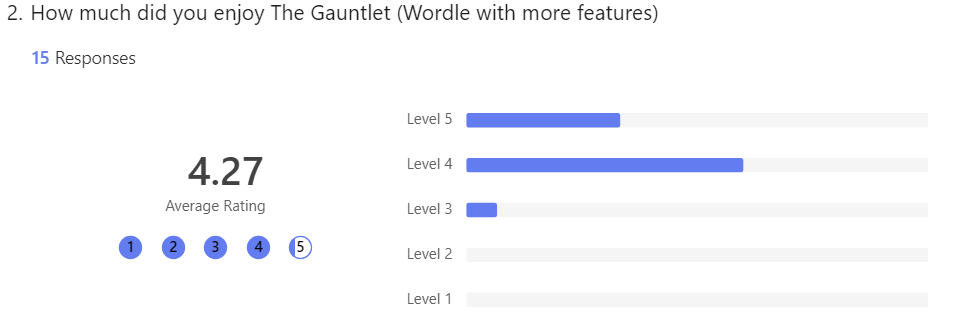
\includegraphics[width=\textwidth]{GauntletResponse1.png} % Replace with your image file
    \label{fig:example}
\end{figure}
\begin{figure}[h] % 'h' means 'here' - places the figure where it's defined
    \centering
    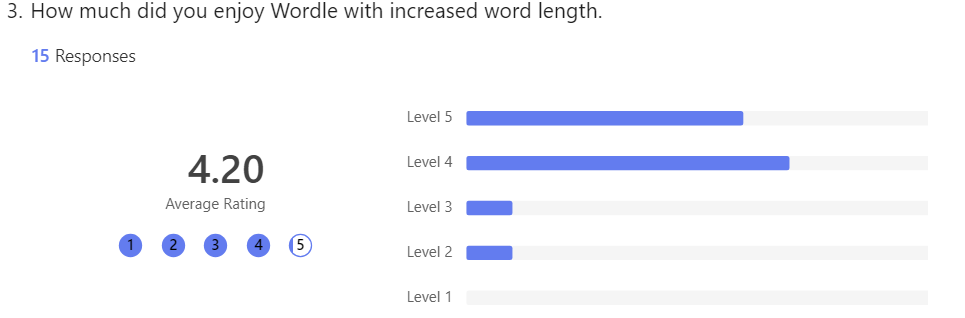
\includegraphics[width=\textwidth]{GauntletResponse2.png} % Replace with your image file
    \label{fig:example}
\end{figure}
\begin{figure}[h] % 'h' means 'here' - places the figure where it's defined
    \centering
    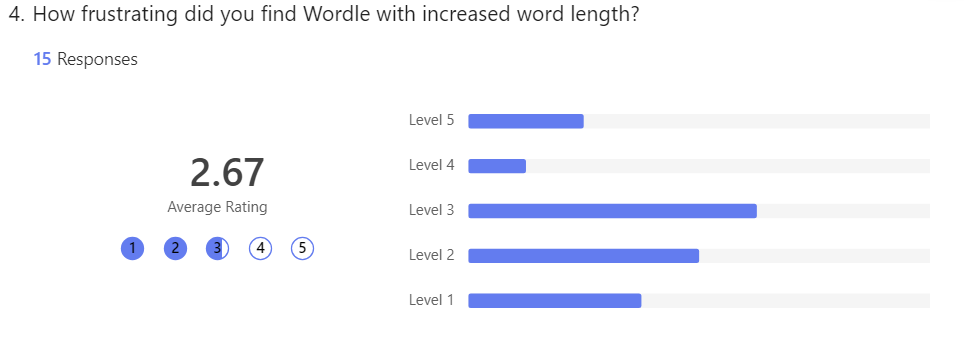
\includegraphics[width=\textwidth]{GauntletResponse3.png} % Replace with your image file
    \label{fig:example}
\end{figure}
\begin{figure}[h] % 'h' means 'here' - places the figure where it's defined
    \centering
    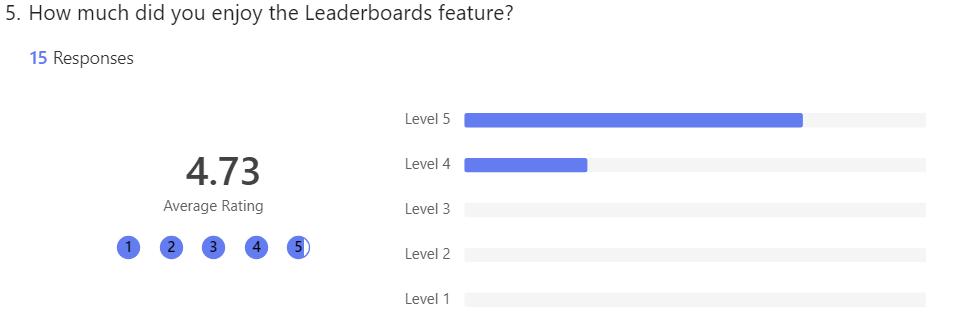
\includegraphics[width=\textwidth]{GauntletResponse4.png} % Replace with your image file
    \label{fig:example}
\end{figure}
\begin{figure}[h] % 'h' means 'here' - places the figure where it's defined
    \centering
    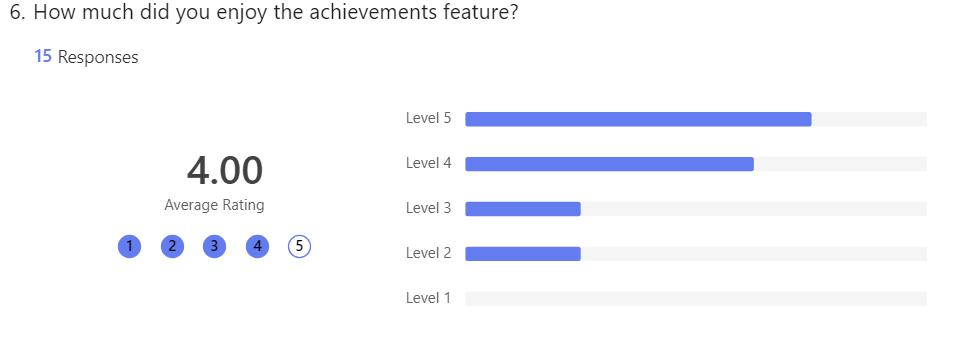
\includegraphics[width=\textwidth]{GauntletResponse5.png} % Replace with your image file
    \label{fig:example}
\end{figure}
\begin{figure}[h] % 'h' means 'here' - places the figure where it's defined
    \centering
    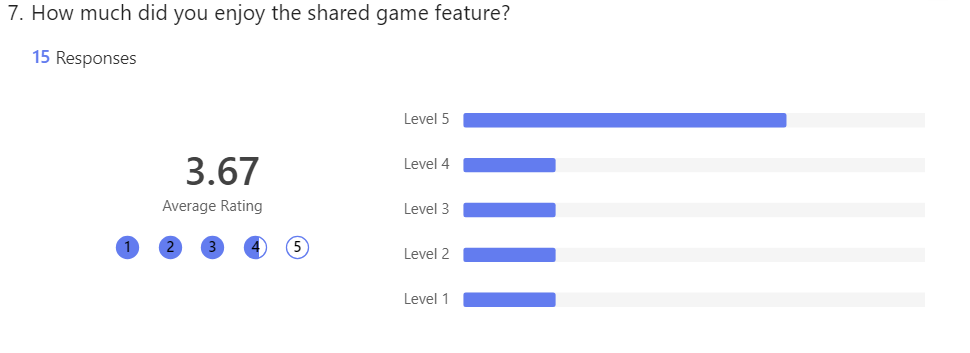
\includegraphics[width=\textwidth]{GauntletResponse6.png} % Replace with your image file
    \label{fig:example}
\end{figure}
\begin{figure}[h] % 'h' means 'here' - places the figure where it's defined
    \centering
    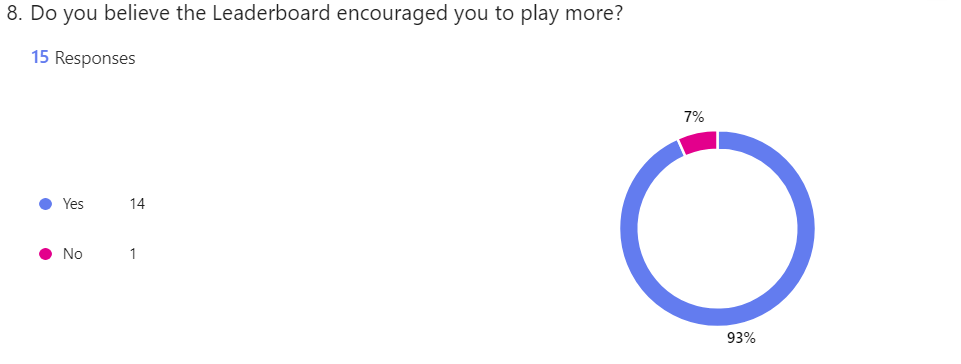
\includegraphics[width=\textwidth]{GauntletResponse7.png} % Replace with your image file
    \label{fig:example}
\end{figure}
\begin{figure}[h] % 'h' means 'here' - places the figure where it's defined
    \centering
    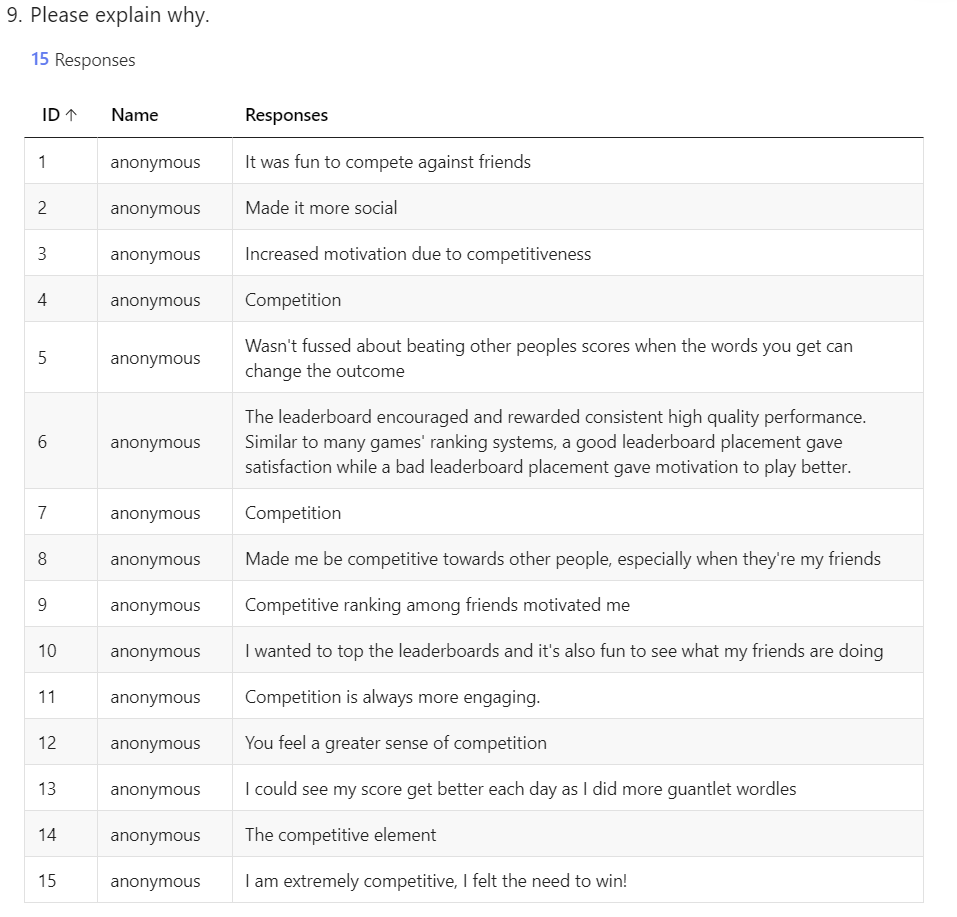
\includegraphics[width=\textwidth]{GauntletResponse8.png} % Replace with your image file
    \label{fig:example}
\end{figure}
\begin{figure}[h] % 'h' means 'here' - places the figure where it's defined
    \centering
    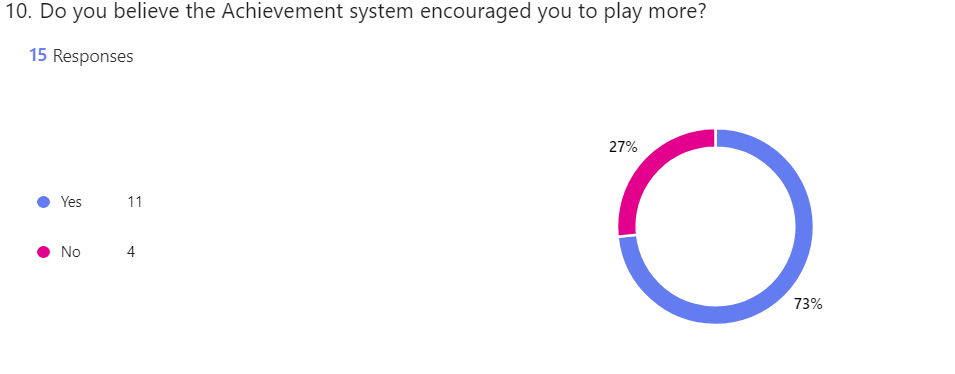
\includegraphics[width=\textwidth]{GauntletResponse9.png} % Replace with your image file
    \label{fig:example}
\end{figure}
\begin{figure}[h] % 'h' means 'here' - places the figure where it's defined
    \centering
    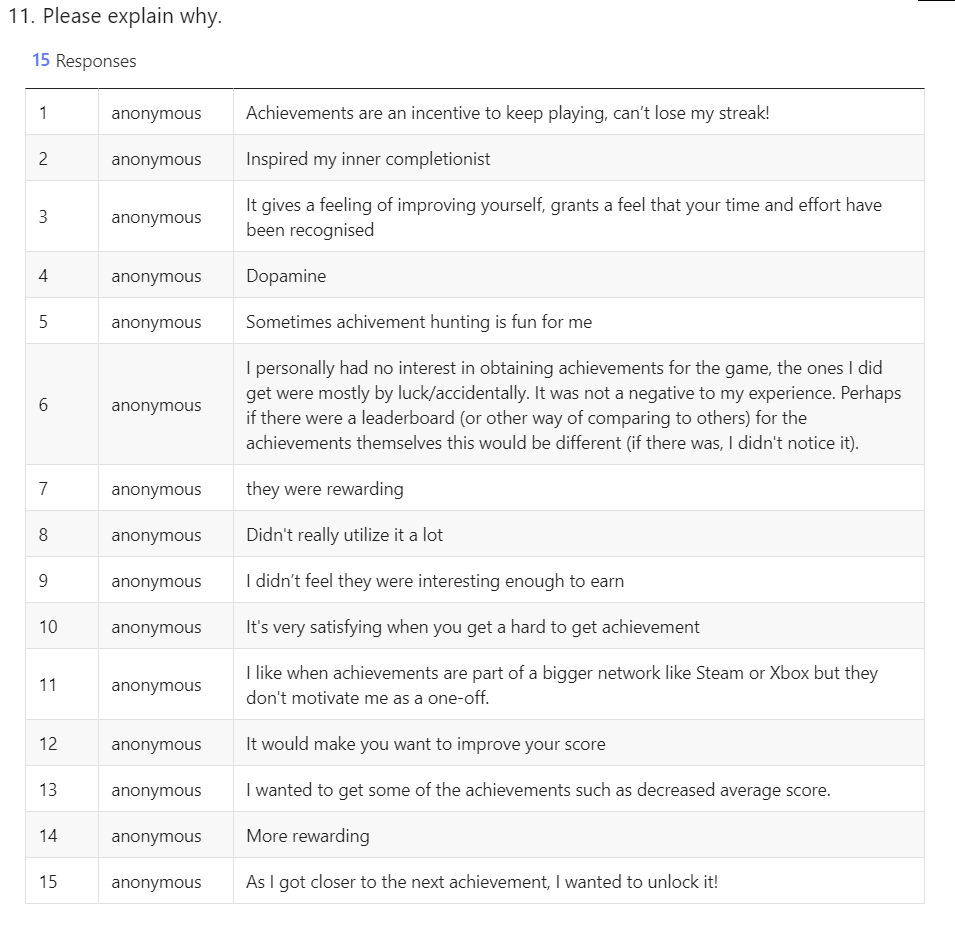
\includegraphics[width=\textwidth]{GauntletResponse10.png} % Replace with your image file
    \label{fig:example}
\end{figure}
\begin{figure}[h] % 'h' means 'here' - places the figure where it's defined
    \centering
    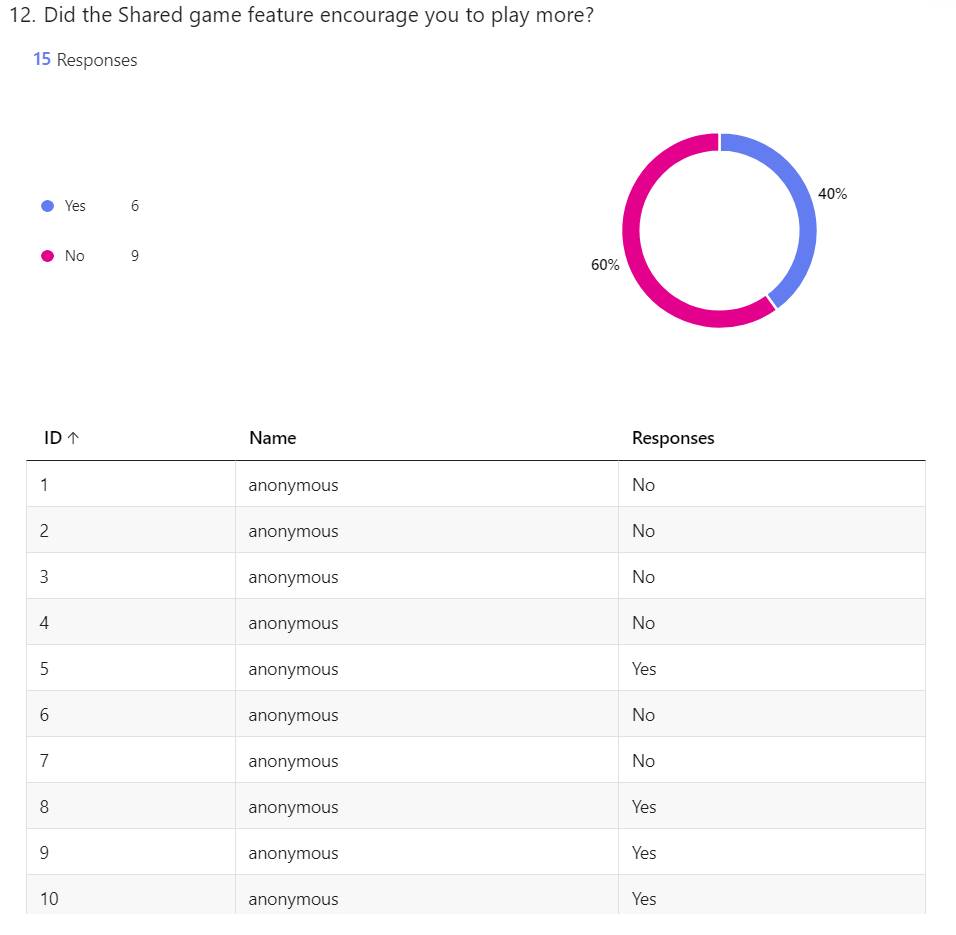
\includegraphics[width=\textwidth]{GauntletResponse11.png} % Replace with your image file
    \label{fig:example}
\end{figure}
\begin{figure}[h] % 'h' means 'here' - places the figure where it's defined
    \centering
    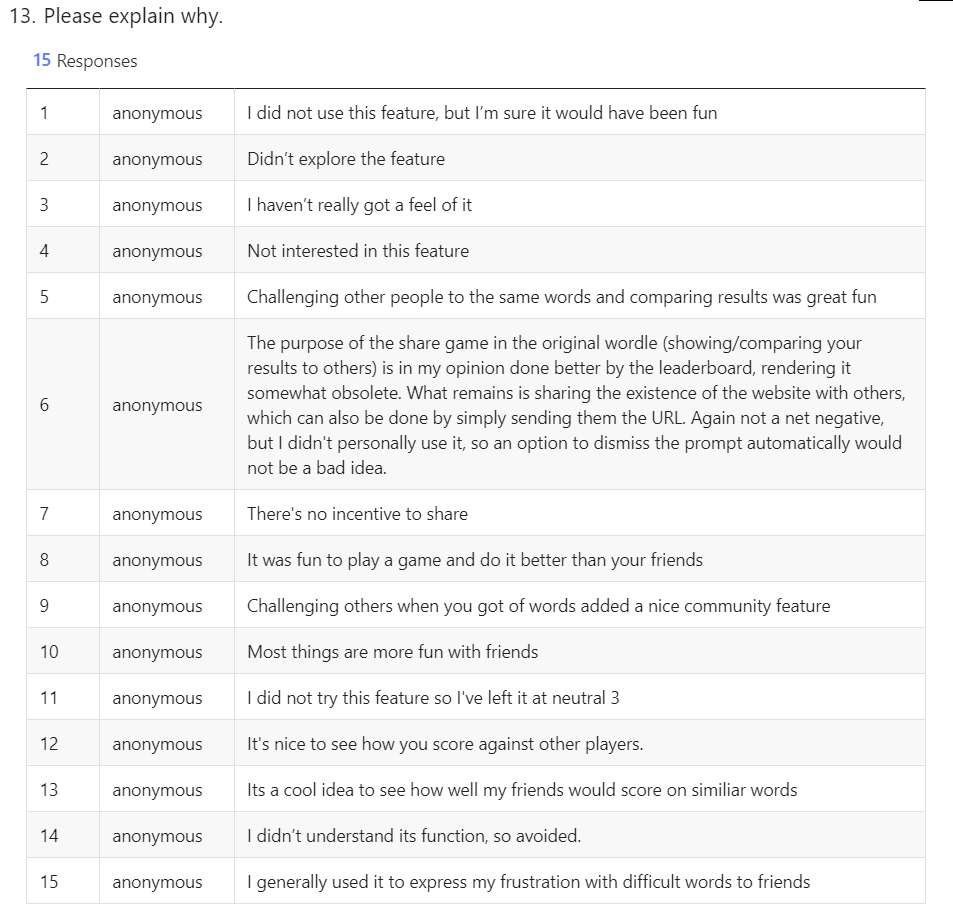
\includegraphics[width=\textwidth]{GauntletResponse12.png} % Replace with your image file
    \label{fig:example}
\end{figure}
\begin{figure}[h] % 'h' means 'here' - places the figure where it's defined
    \centering
    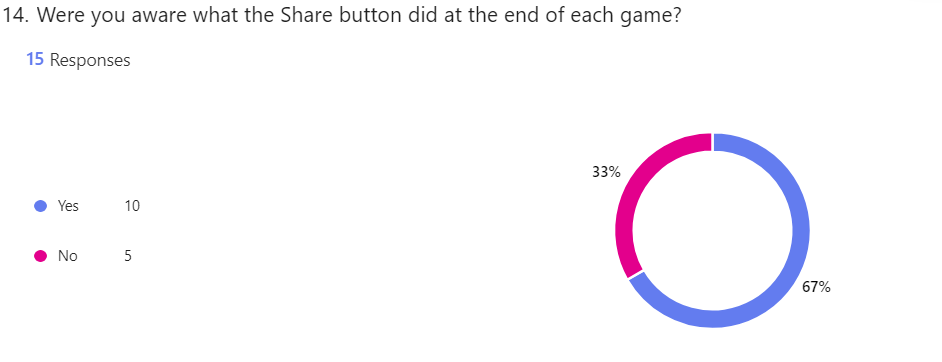
\includegraphics[width=\textwidth]{GauntletResponse13.png} % Replace with your image file
    \label{fig:example}
\end{figure}
\begin{figure}[h] % 'h' means 'here' - places the figure where it's defined
    \centering
    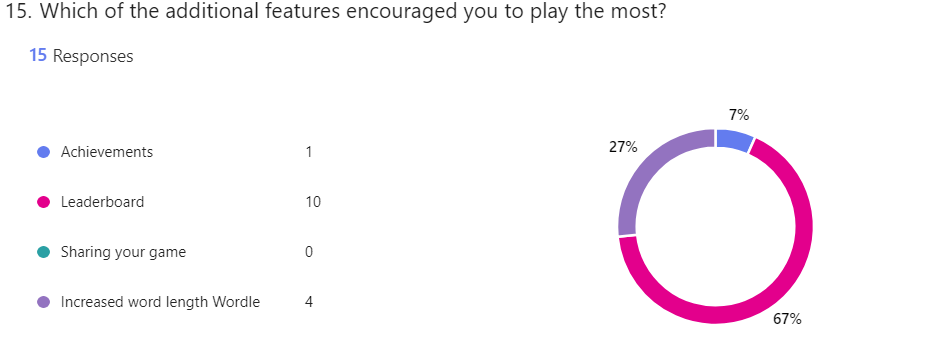
\includegraphics[width=\textwidth]{GauntletResponse14.png} % Replace with your image file
    \label{fig:example}
\end{figure}
\begin{figure}[h] % 'h' means 'here' - places the figure where it's defined
    \centering
    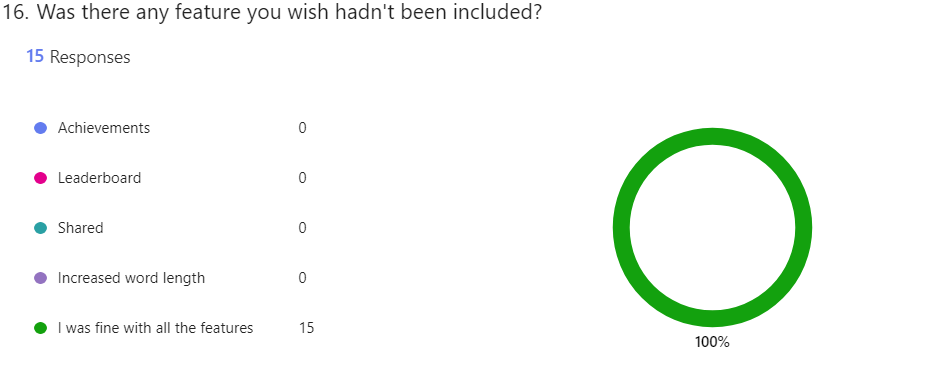
\includegraphics[width=\textwidth]{GauntletResponse15.png} % Replace with your image file
    \label{fig:example}
\end{figure}
\begin{figure}[h] % 'h' means 'here' - places the figure where it's defined
    \centering
    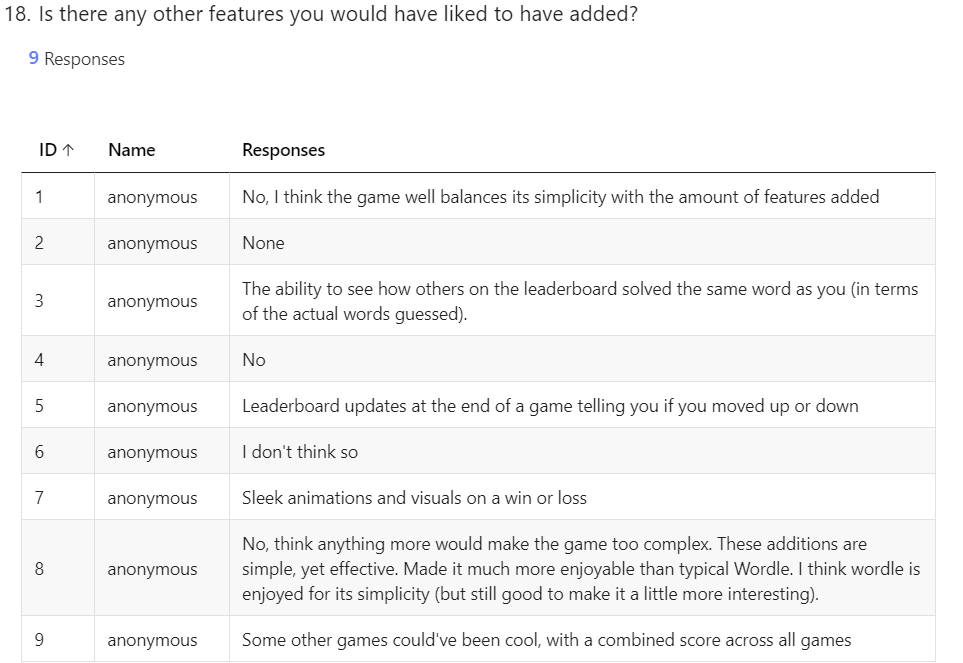
\includegraphics[width=\textwidth]{GauntletResponse16.png} % Replace with your image file
    \label{fig:example}
\end{figure}
\begin{figure}[h] % 'h' means 'here' - places the figure where it's defined
    \centering
    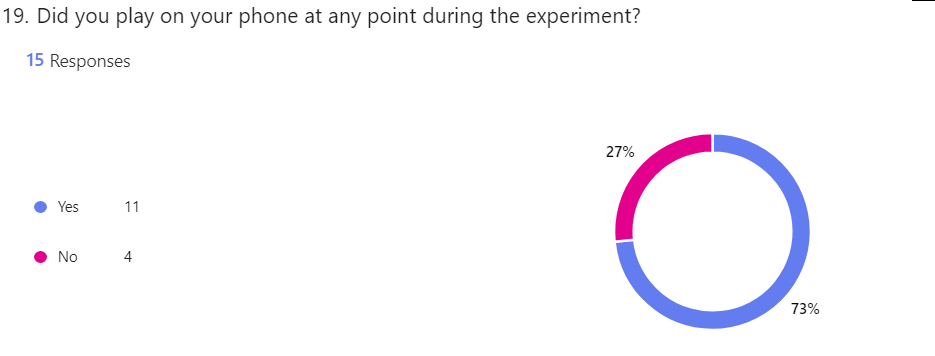
\includegraphics[width=\textwidth]{GauntletResponse17.png} % Replace with your image file
    \label{fig:example}
\end{figure}
\begin{figure}[h] % 'h' means 'here' - places the figure where it's defined
    \centering
    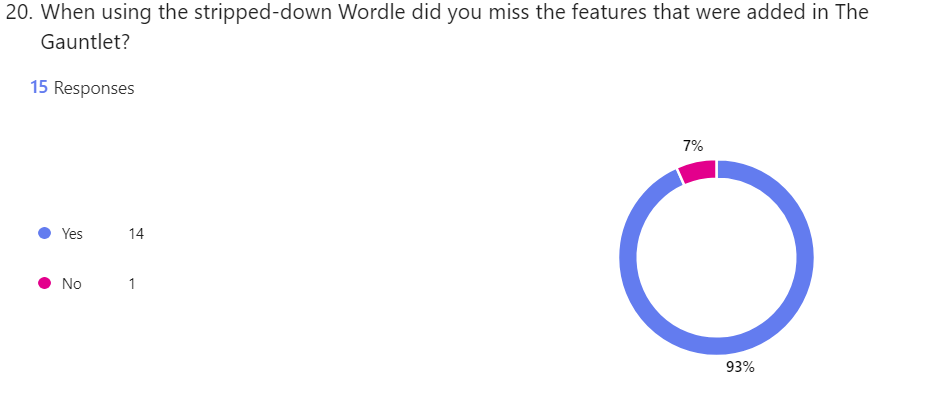
\includegraphics[width=\textwidth]{GauntletResponse18.png} % Replace with your image file
    \label{fig:example}
\end{figure}
\begin{figure}[h] % 'h' means 'here' - places the figure where it's defined
    \centering
    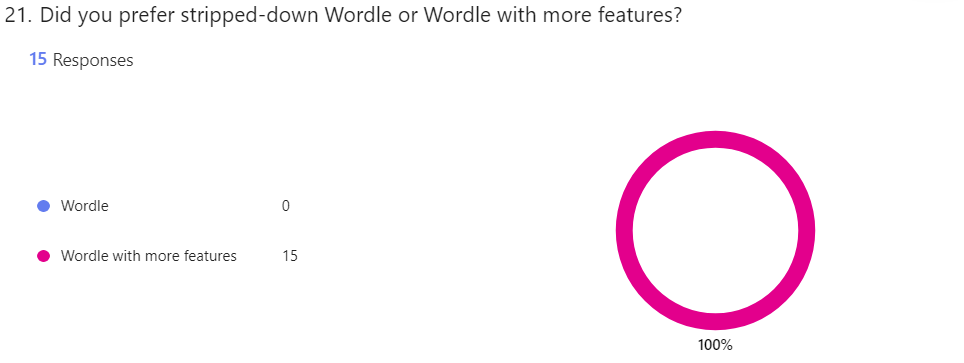
\includegraphics[width=\textwidth]{GauntletResponse19.png} % Replace with your image file
    \label{fig:example}
\end{figure}
\begin{figure}[h] % 'h' means 'here' - places the figure where it's defined
    \centering
    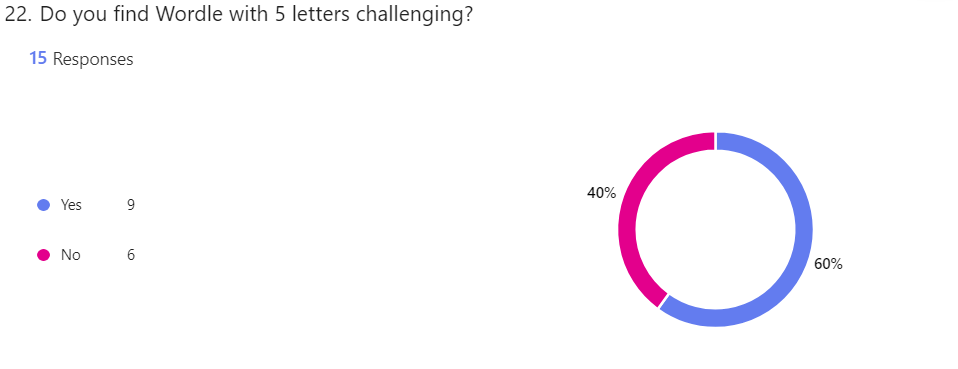
\includegraphics[width=\textwidth]{GauntletResponse20.png} % Replace with your image file
    \label{fig:example}
\end{figure}
\begin{figure}[h] % 'h' means 'here' - places the figure where it's defined
    \centering
    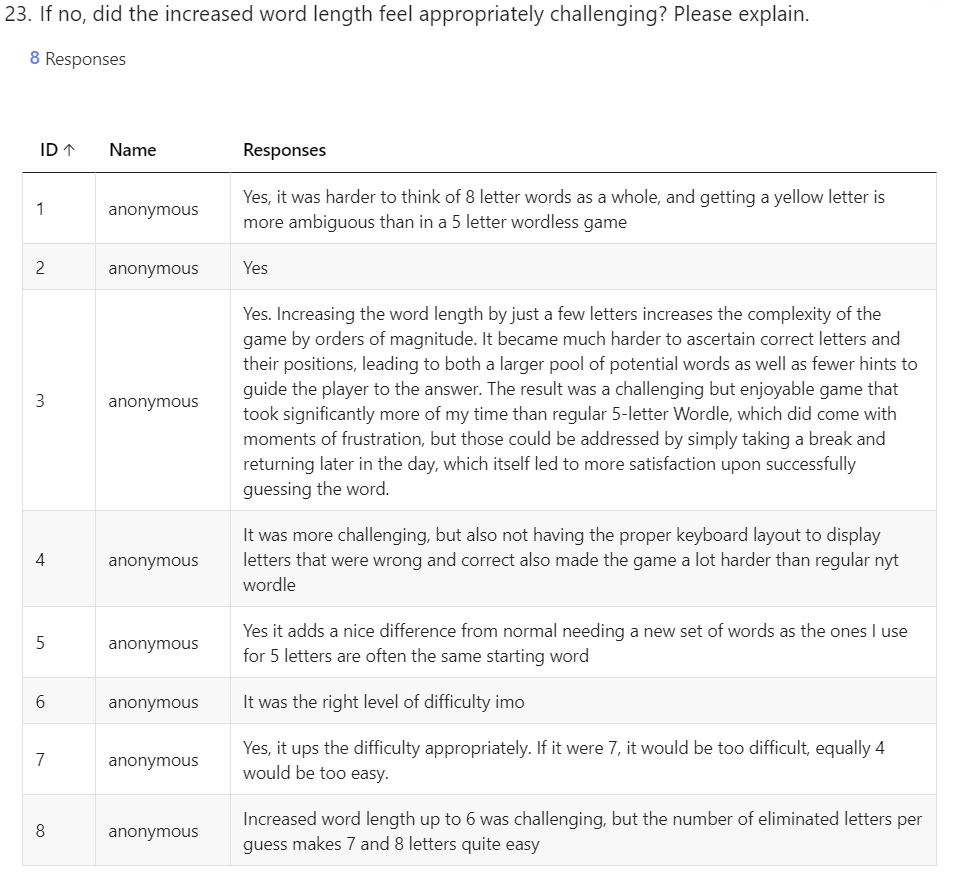
\includegraphics[width=\textwidth]{GauntletResponse21.png} % Replace with your image file
    \label{fig:example}
\end{figure}
\begin{figure}[h] % 'h' means 'here' - places the figure where it's defined
    \centering
    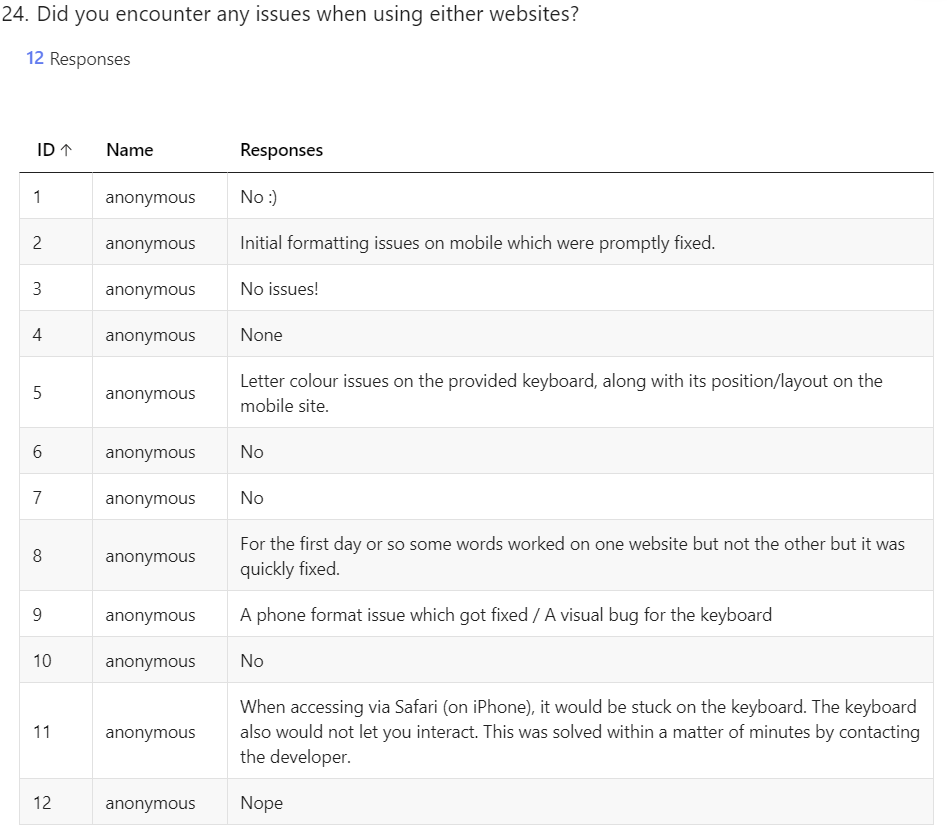
\includegraphics[width=\textwidth]{GauntletResponse22.png} % Replace with your image file
    \label{fig:example}
\end{figure}
\clearpage

\section{Google Analytics Result}
\begin{figure}[h] % 'h' means 'here' - places the figure where it's defined
    \centering
    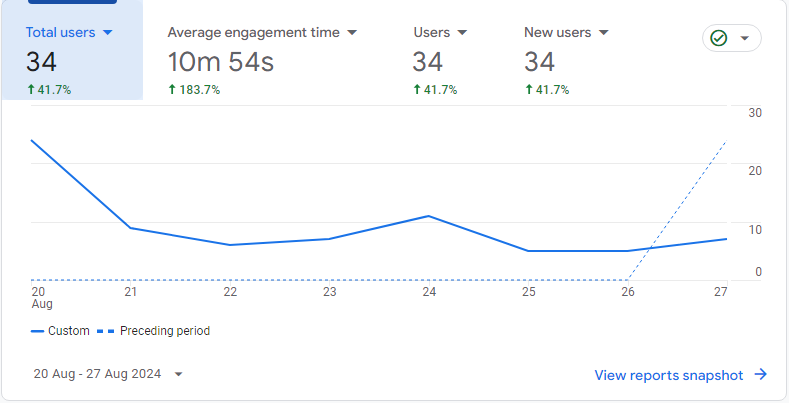
\includegraphics[width=\textwidth]{GoogleAnalytics1.png} % Replace with your image file
    \label{fig:example}
    \caption{Graph of the total users each day for The Gauntlet}
\end{figure}
\begin{figure}[h] % 'h' means 'here' - places the figure where it's defined
    \centering
    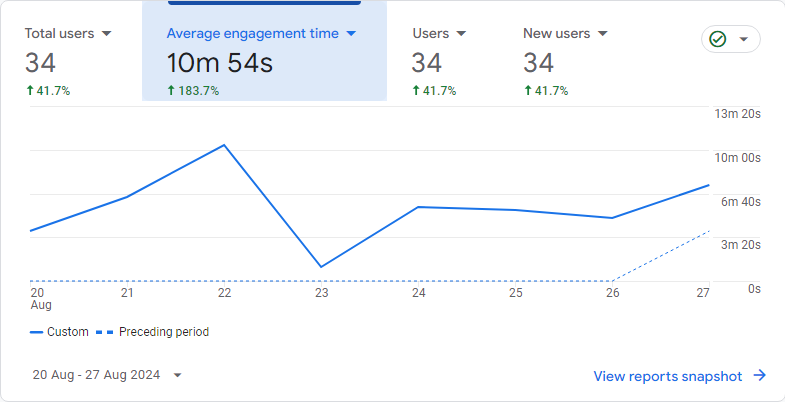
\includegraphics[width=\textwidth]{GoogleAnalytics2.png} % Replace with your image file
    \label{fig:example}
    \caption{Graph of average engagement time each day for The Gauntlet}
\end{figure}
\begin{figure}[h] % 'h' means 'here' - places the figure where it's defined
    \centering
    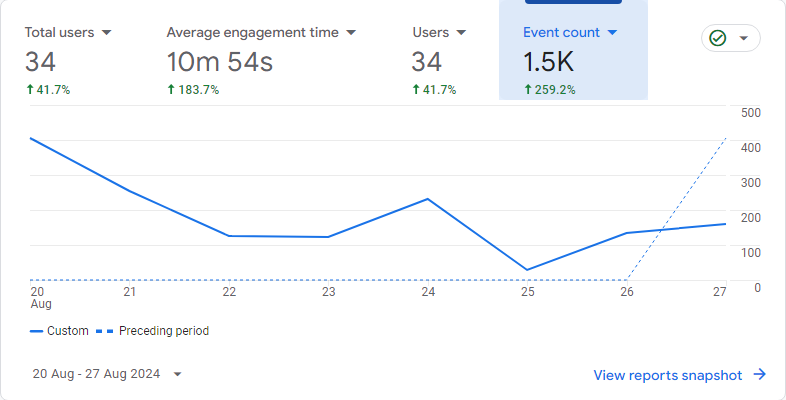
\includegraphics[width=\textwidth]{GoogleAnalytics3.png} % Replace with your image file
    \label{fig:example}
    \caption{Graph of event count each day for The Gauntlet}
\end{figure}
\begin{figure}[h] % 'h' means 'here' - places the figure where it's defined
    \centering
    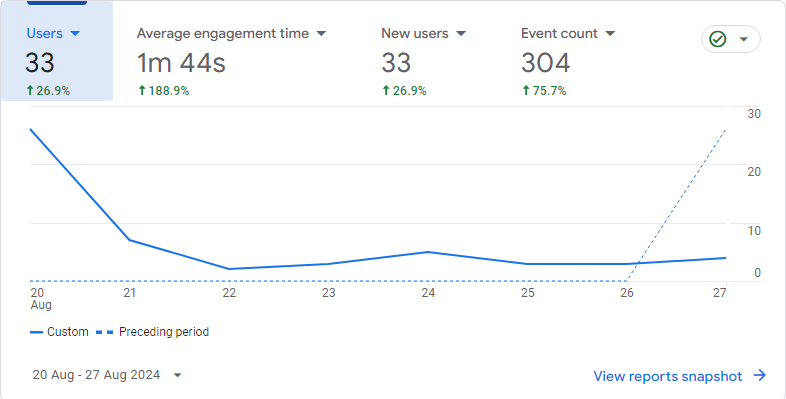
\includegraphics[width=\textwidth]{GoogleAnalytics4.png} % Replace with your image file
    \label{fig:example}
    \caption{Graph of total users each day for Wordle no-login}
\end{figure}
\begin{figure}[h] % 'h' means 'here' - places the figure where it's defined
    \centering
    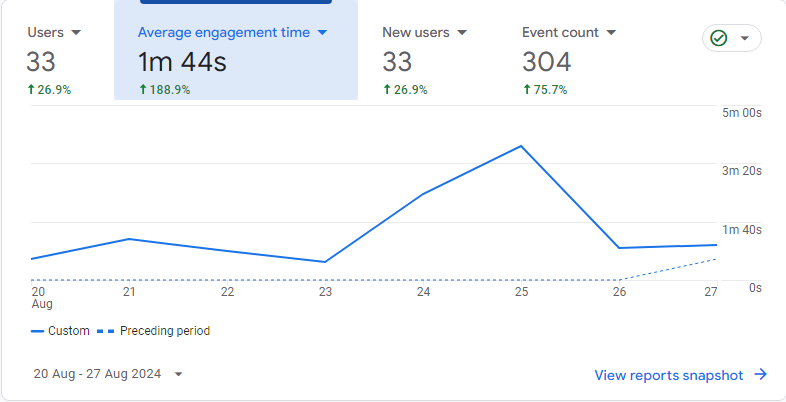
\includegraphics[width=\textwidth]{GoogleAnalytics5.png} % Replace with your image file
    \label{fig:example}
    \caption{Graph of average engagement time each day for Wordle no-login}
\end{figure}
\begin{figure}[h] % 'h' means 'here' - places the figure where it's defined
    \centering
    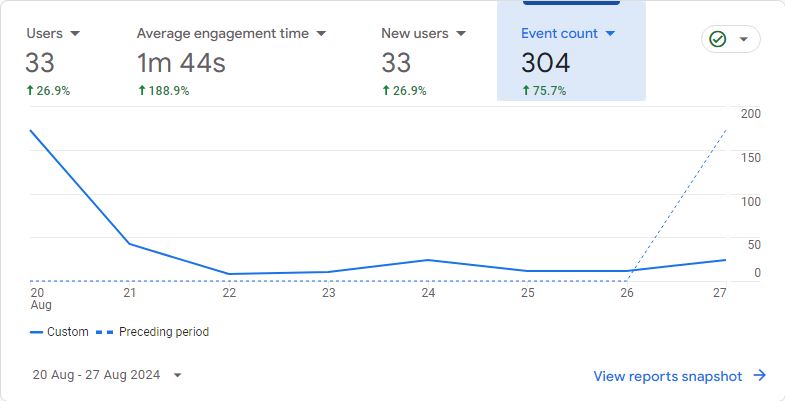
\includegraphics[width=\textwidth]{GoogleAnalytics6.png} % Replace with your image file
    \label{fig:example}
    \caption{Graph of event count each day for Wordle no-login}
\end{figure}

\end{document}
